%----------------------------------------------------------------------------------------
%	PACKAGES AND THEMES
%----------------------------------------------------------------------------------------

\documentclass[compress]{beamer}

\mode<presentation> {

% The Beamer class comes with a number of default slide themes
% which change the colors and layouts of slides. Below this is a list
% of all the themes, uncomment each in turn to see what they look like.

%\usetheme{default}
%\usetheme{AnnArbor}
\usetheme{Antibes}
%\usetheme{Bergen}
%\usetheme{Berkeley}
%\usetheme{Berlin}
%\usetheme{Boadilla}
%\usetheme{CambridgeUS}
%\usetheme{Copenhagen}
%\usetheme{Darmstadt}
%\usetheme{Dresden}
%\usetheme{Frankfurt}
%\usetheme{Goettingen}
%\usetheme{Hannover}
%\usetheme{Ilmenau}
%\usetheme{JuanLesPins}
%\usetheme{Luebeck}
%\usetheme{Madrid}
%\usetheme{Malmoe}
%\usetheme{Marburg}
%\usetheme{Montpellier}
%\usetheme{PaloAlto}
%\usetheme{Pittsburgh}
%\usetheme{Rochester}
%\usetheme{Singapore}
%\usetheme{Szeged}
%\usetheme{Warsaw}


% As well as themes, the Beamer class has a number of color themes
% for any slide theme. Uncomment each of these in turn to see how it
% changes the colors of your current slide theme.

%\usecolortheme{albatross}
%\usecolortheme{beaver}
%\usecolortheme{beetle}
%\usecolortheme{crane}
%\usecolortheme{dolphin}
%\usecolortheme{dove}
%\usecolortheme{fly}
%\usecolortheme{lily}
%\usecolortheme{orchid}
%%\usecolortheme{rose}
%\usecolortheme{seagull}
%\usecolortheme{seahorse}
%%\usecolortheme{whale}
%\usecolortheme{wolverine}
%\usecolortheme{structure}

\usefonttheme[onlylarge]{structurebold}
\useinnertheme{circles}
\useoutertheme[subsection=false]{miniframes}
\setbeamertemplate{headline}{}

\setbeamertemplate{blocks}[rounded]

%\setbeamertemplate{footline} % To remove the footer line in all slides uncomment this line
%\setbeamertemplate{footline}% To replace the footer line in all slides with a simple slide count uncomment this line
                  {
                    \insertshortauthor[center]
                    }
\setbeamertemplate{caption}[]
\setbeamertemplate{itemize item}{\textbullet}
\setbeamertemplate{navigation symbols}{} % To remove the navigation symbols from the bottom of all slides uncomment this line
}

\usepackage[utf8]{inputenc}
%\usepackage[portuguese]{babel}
\usepackage{hyphenat}
\hyphenation{im-ple-men-ta-cao}

\usepackage{siunitx}
\usepackage{xmpmulti}
\usepackage{geometry}
\usepackage{multimedia}
\usepackage{ragged2e}
\usepackage{etoolbox}
\usepackage{color}
\usepackage{tabto}
\usepackage{alltt}
\usepackage{gensymb}
\usepackage{esvect}
\usepackage{soul}
\usepackage{courier}
\usepackage{amsmath}
\usepackage{mathtools}

\definecolor{dgreen}{rgb}{0.,0.6,0.}
\definecolor{grey}{rgb}{0.55,0.55,0.55}
\definecolor{dyellow}{RGB}{153,153,0}
\definecolor{byellow}{RGB}{120,120,0}

\usepackage{graphicx}
\usepackage{booktabs} 
\usepackage{multicol}
\usepackage{vwcol} 
\usepackage{multirow}

%----------------------------------------------------------------------------------------
%	TITLE PAGE
%----------------------------------------------------------------------------------------

\title[Short title]{Data Science Course\\
\small{Understading swarm behaviour}}
\vspace*{-30pt}\titlegraphic{
\includegraphics[width=5cm]{./img/FUB_logo.png}}

\author[Grupo B4]{Felicia Burtscher, Frederik Eistrup, Jos\'{e} Senart\\  %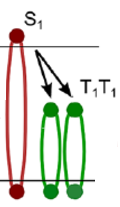
\includegraphics[width=0.15\columnwidth]{../img/SF_linda.pdf}\\
%\includegraphics[width=0.15\columnwidth]{../img/LBIC_CELLO_fig5.png}\includegraphics[width=0.15\columnwidth]{../img/LBIC_CELLO_fig9.png}
} % Your name

%\vspace{10pt}
%\includegraphics[width=0.2\columnwidth]{../img/LBIC_CELLO_fig9.png}\\

%\textit{"The imagination of nature is far, far greater than the imagination of man."} 
%, Richard Feynman}
%\textit{"Not everything that counts can be counted, \\and not everything that can be counted counts"}\\ Albert Einstein}
\date{\today} 
\institute[FUB]{\vspace{-10pt}Freie Universität Berlin}
%	\centering
\begin{document}

\begin{frame}
\titlepage
\end{frame}

%\begin{frame}\footnotesize
%\frametitle{Índice} % Table of contents slide, comment this block out to remove it
%\tableofcontents % Throughout your presentation, if you choose to use \section{} and \subsection{} commands, these will automatically be printed on this slide as an overview of your presentation
%\normalsize
%\end{frame}

%----------------------------------------------------------------------------------------
%	PRESENTATION SLIDES
%----------------------------------------------------------------------------------------

\begin{frame}
  \frametitle{Presentation Overview}

  \begin{itemize}
  	\item All models: sim300.py
	\item Paper 1: Effective leadership and decision-making in animal groups on the move (Couzin et al)
	\item Paper 2: Double milling in self-probelled swarms from kinetic theory (Carrillo et al)
	\item Quantification
  \end{itemize}


 % \end{multicols}
\end{frame}

\begin{frame}
  \frametitle{All models: sim300.py}
  
  
  \texttt{
  Models available:\\
  'Simple speed coupling..................smpl'
  'Couzin model...........................czn'
  'Viscek model...........................vsck'
  'Couzin-2 model.........................czn2'
  'Mill model.............................mill'
}
  
   
%Photovoltaics efficiency from Solar Spectrum is limited (Shockley-Queisser Limit $\sim 34\%$)\\
%\begin{multicols}{2}
%%\hspace{-10pt}
%\begin{figure}[H]
%%centering
%	\hspace{-20pt} 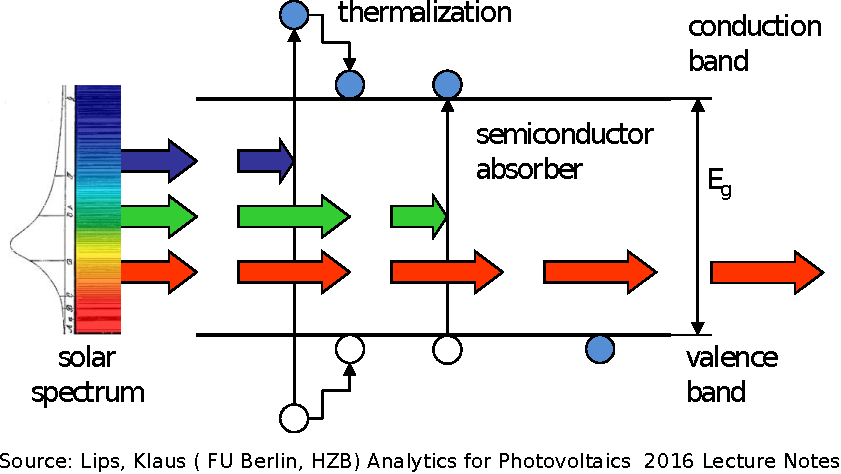
\includegraphics[width=1.15\columnwidth]{../img/SF_esq14.pdf}
%\end{figure}
%\begin{figure}[H]
%%	\centering
%\hspace{60pt}	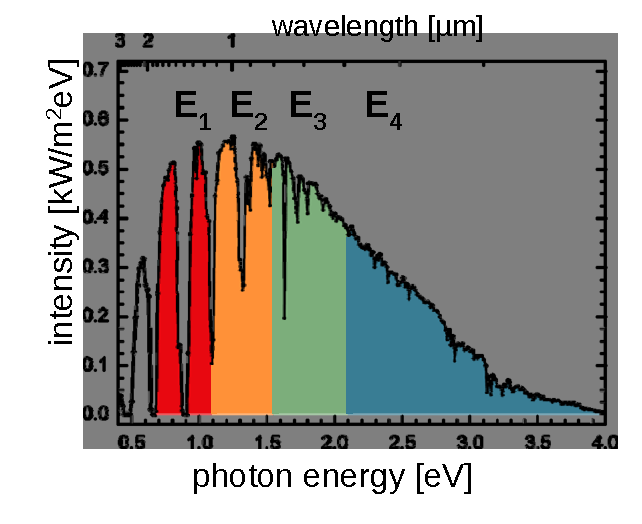
\includegraphics[width=.85\columnwidth]{../img/SF_esq16.pdf}
%\end{figure}
%
%\end{multicols}
%
%
%\begin{multicols}{2}
%Wasted Energy\\
% $\rightarrow$ Possible to collect?\\
%\columnbreak
%Solutions:\\
%
%- \st{Non-Linear Optics} ($\omega'=2\omega$)\\
%- Multi-layer design\\
%- Up- \& Down-Conversion
%\end{multicols}
\end{frame}

\begin{frame}
  \frametitle{Paper 1: Effective leadership and decision-making in animal groups on the move (Couzin et al): \texttt{czn2}}
 
 same as Couzin 1 model but without orientation phase
%\small
%\begin{multicols}{2}
%\begin{figure}[H]
%%centering
%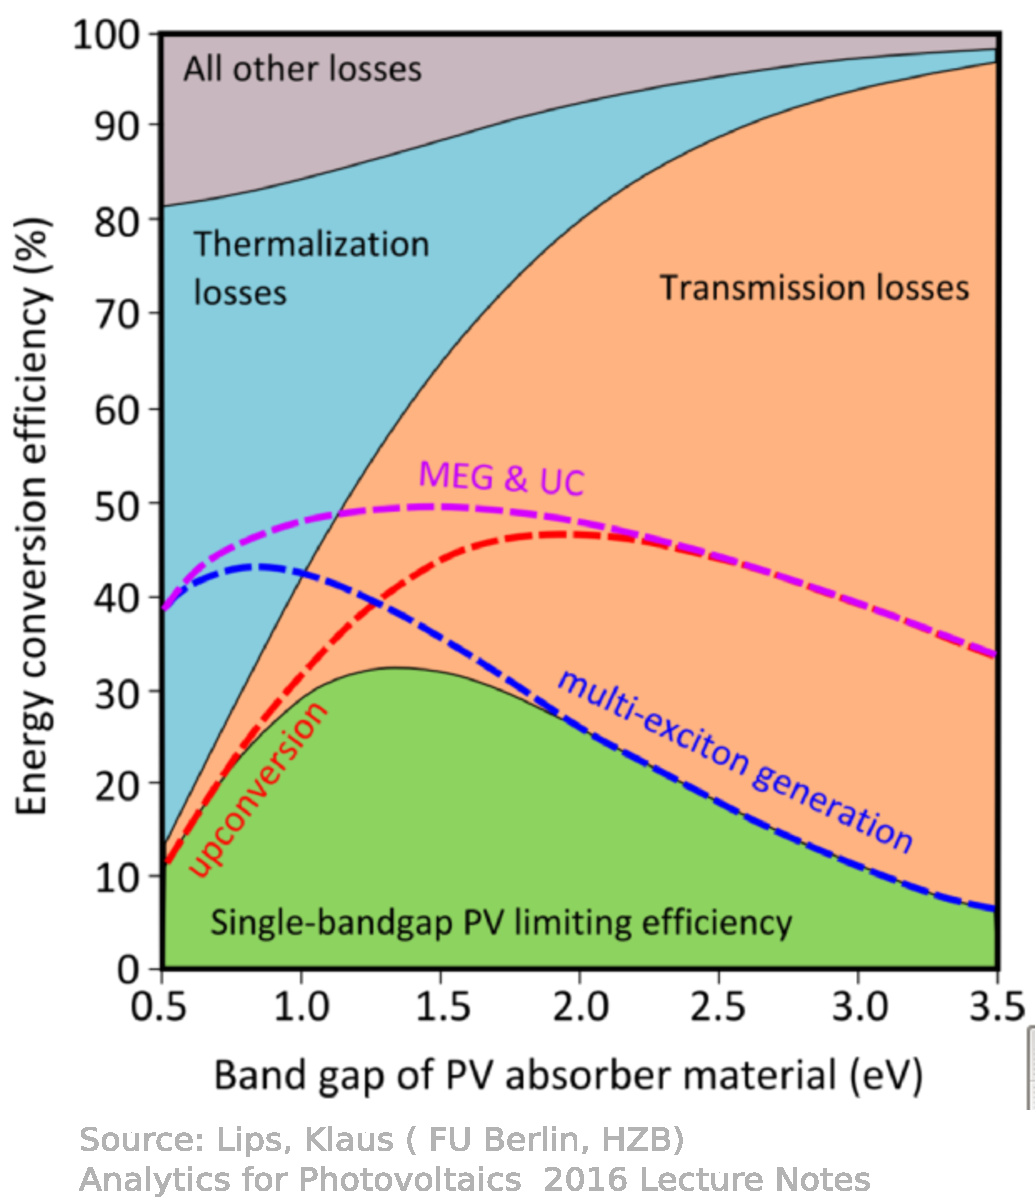
\includegraphics[width=1\columnwidth]{../img/SF_esq17.pdf}
%\end{figure}
%\columnbreak
%
%\underline{Up-Conversion} (UC)\\
%low E photons \textbf{added} to $E_g$\\
%$\rightarrow$ Triplet-Triplet Annihilation (TTA)\\
%%picture w/ band diagram UC
%
%\vspace{10pt}
%
%\underline{Down-Conversion} (DC)\\
%high E photons \textbf{split} to $E_g$\\
%\footnotesize(Multi-Exciton Generation (MEG))\\
%\small
%$\rightarrow$ Quantum Dots (inorganic)\\
%\begin{multicols}{2}
%\vspace{-30pt}\begin{figure}[H]
%\vspace{-10pt}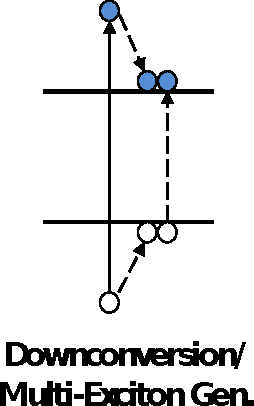
\includegraphics[width=0.6\columnwidth]{../img/SF_esq12.pdf}
%\end{figure}
%\hspace{-10pt}$\rightarrow$\textbf{Singlet-Fission (SF)} (organic) \\
%
%\end{multicols}
%
%\end{multicols}
\end{frame}


\begin{frame}
  \frametitle{Paper 2: Double milling in self-probelled swarms from kinetic theory (Carrillo et al): \texttt{mill}}
\small A kinetic theory based approach for swarming systems of self-propelled discrete particles. \\

%Models to describe a collection of interacting agents as discrete particles or as a continuous density

  Individuals driven by self-propelling forces and pairwise attractive and repulsive interactions lead to various morphologies, e.f. flocks, rotating mills, rings and clumps. \\
  We can \\
  - average in direction or velocity \\
  - consider different zones of interaction and averaging (see Couzin et al)
  

%\begin{multicols}{2}
%
%\begin{figure}[H]
%%centering
%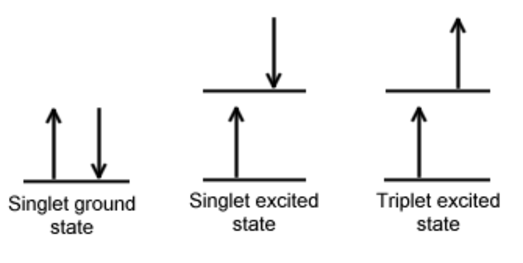
\includegraphics[width=1\columnwidth]{../img/SF_esq7.pdf}
%\end{figure}
%
%- $T_1$ lower than $S_1$ due to exchange interaction (we need $2E_{T1}\simeq E_{S1}$)\\
%- \textbf{Spin Conservation} \underline{disallows} competing thermal relaxation\\
%\end{multicols}
%
%\begin{figure}[H]
%%centering
%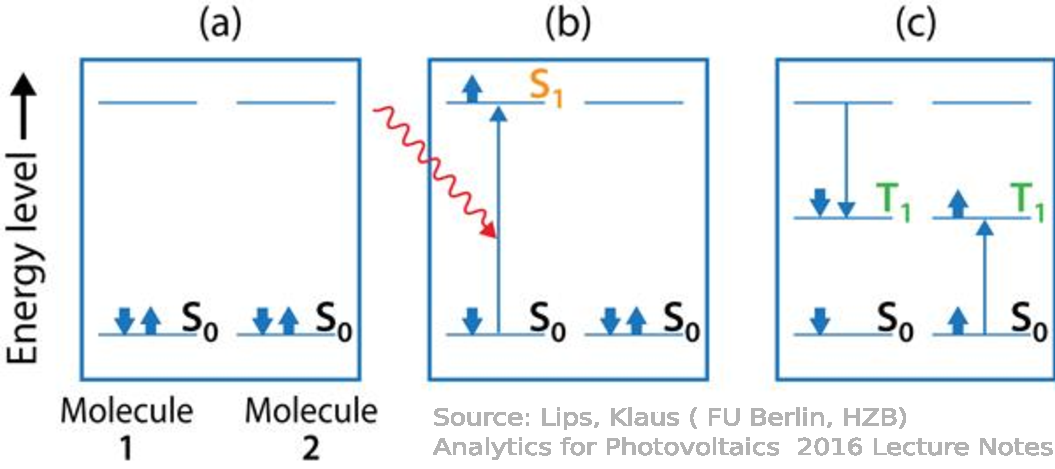
\includegraphics[width=1\columnwidth]{../img/SF_esq9.pdf}
%\end{figure}


\end{frame}

\begin{frame}
	\frametitle{Paper 2: Double milling in self-probelled swarms from kinetic theory (Carrillo et al): \texttt{mill}}
	
	  
	  But: As N=#particles grows, it becomes increasingly difficult to follows the dynamics of each individual agent. Therefore, we choose a continuous approach where particles are represented by a density field. \\
	  
	%\textbf{Discrete model}: \\ \\
	Consider \( N \) interacting, self-propelled particles governed by the following equations of motion
	
	
	\begin{equation} \label{eqOfMotion}
	\begin{split}
    & \frac{\partial \vec{x_{i}}}{\partial t} = \vec{v_{i}} \\
	m & \frac{\partial \vec{v_{i}}}{\partial t} = (\alpha - \beta |\vec{v_{i}}|^{2}) \vec{v_{i}} - \vec{\nabla_{i}} U(\vec{x_{i}})
	\end{split}
	\end{equation}
	
	where \( U \) is a pairwise interaction potential and \( \alpha, \beta > 0\) are values for propulsion and friction forces.\\

\end{frame}


\begin{frame}
	\frametitle{Paper 2: Double milling in self-probelled swarms from kinetic theory (Carrillo et al): \texttt{mill}}
	

For \( U \) we choose the \textit{Morse potential} which is a common choice for interacting swarming systems

\begin{equation} \label{morsePotential}
U(\vec{x_{i}}) = \sum_{j \neq i}^{} [ \underbrace{-C_{a} e^{-| \vec{x_{i}} - \vec{x_{j}} | / l_{a}}}_{\text{attraction}} + \underbrace{C_{r}e^{-|\vec{x_{i}}-\vec{x_{j}}|/l_{r}}}_{\text{repulsion}} ]
\end{equation}
where \( C_{a}\), \( C_{r}\) denote attractive and repulsive strengths and \( l_{a}\), \( l_{r}\) their respective length scales.
	
\end{frame}

\begin{frame}
  \frametitle{Quantification}
%%\begin{multicols}{2}
%\begin{figure}[H]
%\hspace{-10pt}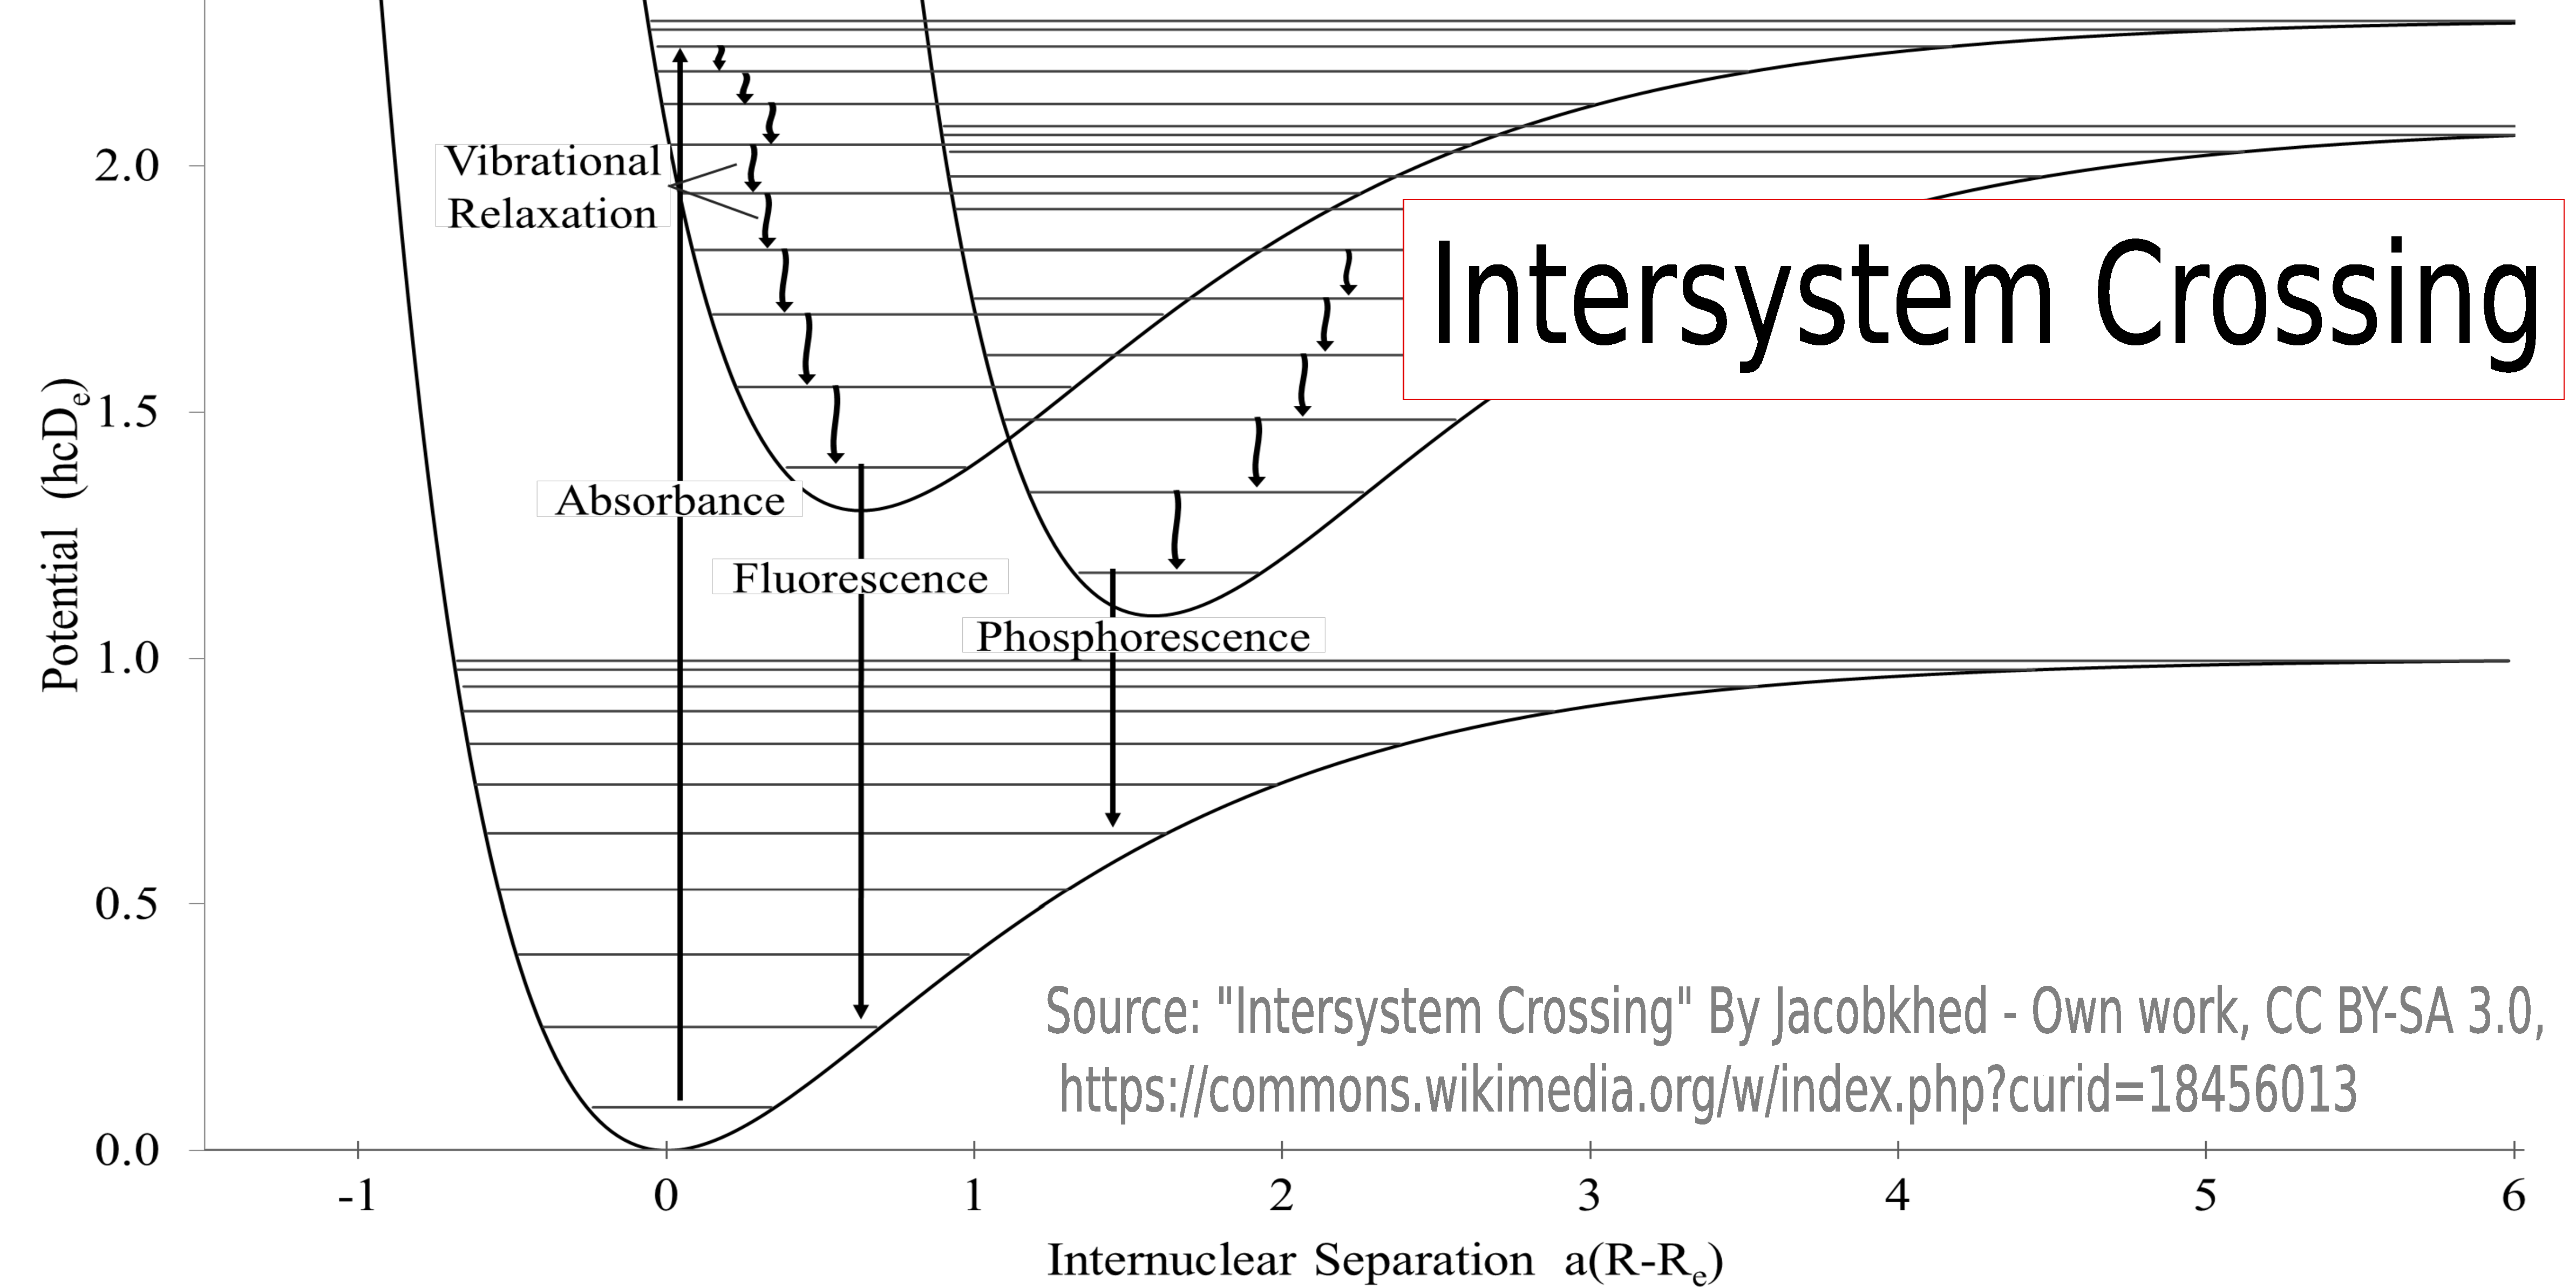
\includegraphics[width=0.9\columnwidth]{../img/SF_esq20.pdf}
%\end{figure}
%\begin{multicols}{2}
%
%\hspace{-20pt}\vspace{-20pt}
%\begin{figure}[H]
%\hspace{-20pt}\vspace{-20pt}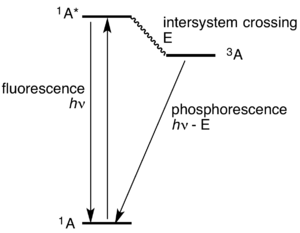
\includegraphics[width=0.7\columnwidth]{../img/SF_esq19.png}
%\end{figure}
%%\columnbreak
%\footnotesize
%\hspace{-20pt}Non-Radiatively: Singlet to Triplet state (reverse of the electron spin)\\
%\hspace{-20pt}1- Overlap of vibrational levels\\
%(little E loss/gain, $\sim kT$)\\
%\hspace{-20pt}2- \textbf{Spin-Orbit Coupling}\\
%%(Interaction with $\overrightarrow{L}$ of non-circular orbits)\\
%%\hspace{-20pt}
%(heavy-atom molecules and paramagnetic species)
%
%\end{multicols}
\end{frame}


\begin{frame}
	\frametitle{Quantification \texttt{czn2}}
Figure 1: Accuracy 
\end{frame}

\begin{frame}
	\frametitle{Quantification \texttt{czn2}}
	Figure 2: Group elongation 
\end{frame}

\begin{frame}
	\frametitle{Quantification \texttt{czn2}}
	Figure 3: Two groups
\end{frame}


\begin{frame}
	\frametitle{Quantification \texttt{mill}}
	
	\begin{figure}[H]
		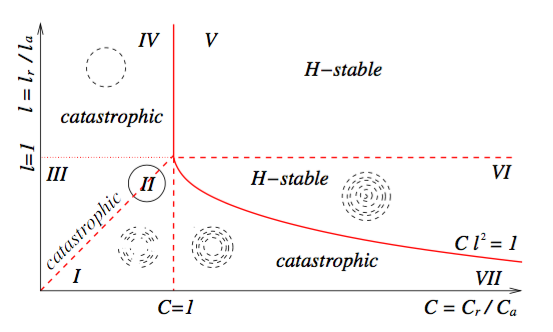
\includegraphics[width=1.\columnwidth]{./img/H-stabilityPhaseDiagram.png}
		\caption{H-stability phase diagram of the Morse potential}
		\label{hstability}
	\end{figure}
	
	
	%%\begin{multicols}{2}
	%\begin{figure}[H]
	%\hspace{-10pt}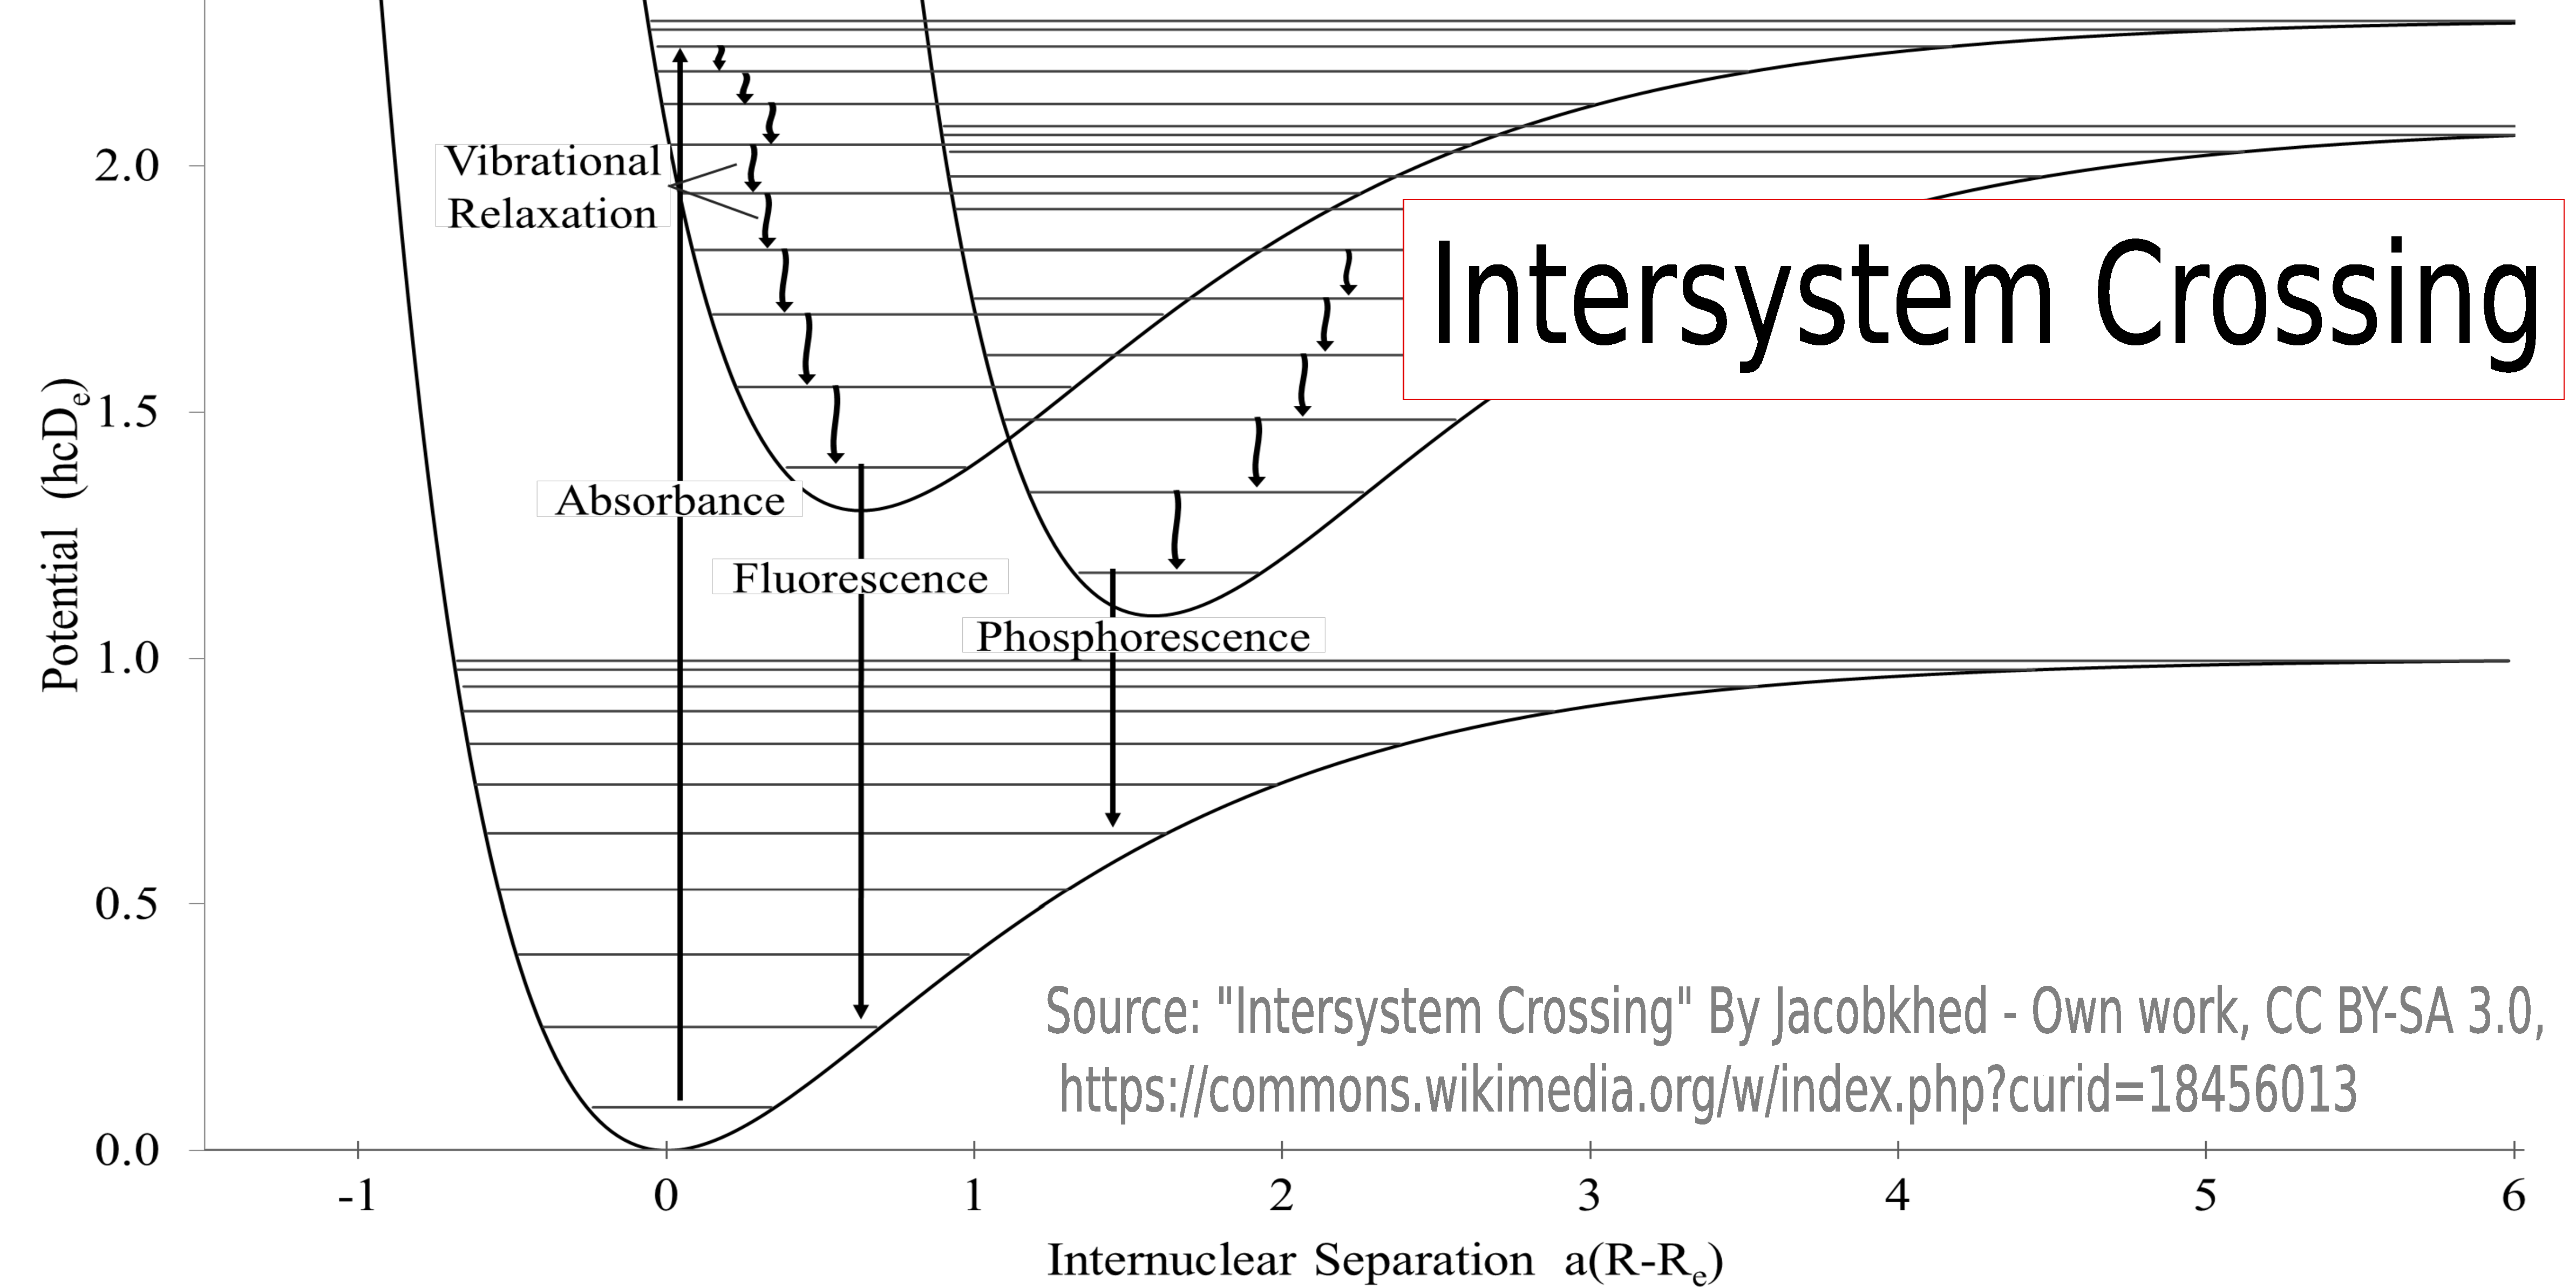
\includegraphics[width=0.9\columnwidth]{../img/SF_esq20.pdf}
	%\end{figure}
	%\begin{multicols}{2}
	%
	%\hspace{-20pt}\vspace{-20pt}
	%\begin{figure}[H]
	%\hspace{-20pt}\vspace{-20pt}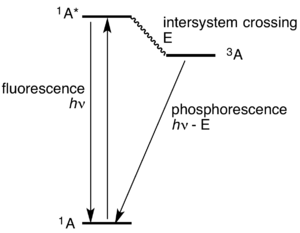
\includegraphics[width=0.7\columnwidth]{../img/SF_esq19.png}
	%\end{figure}
	%%\columnbreak
	%\footnotesize
	%\hspace{-20pt}Non-Radiatively: Singlet to Triplet state (reverse of the electron spin)\\
	%\hspace{-20pt}1- Overlap of vibrational levels\\
	%(little E loss/gain, $\sim kT$)\\
	%\hspace{-20pt}2- \textbf{Spin-Orbit Coupling}\\
	%%(Interaction with $\overrightarrow{L}$ of non-circular orbits)\\
	%%\hspace{-20pt}
	%(heavy-atom molecules and paramagnetic species)
	%
	%\end{multicols}
\end{frame}



\begin{frame}
	\frametitle{Quantification \texttt{mill}}
	
%\begin{figure}[H]
%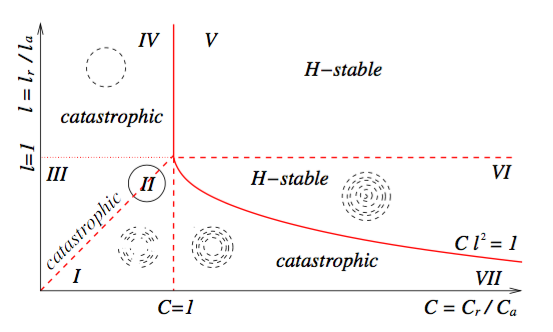
\includegraphics[width=1.\columnwidth]{./img/H-stabilityPhaseDiagram.png}
%\caption{H-stability phase diagram of the Morse potential}
%\label{hstability}
%\end{figure}
%	

Region I \\
Region II \\
Region III \\
Region IV \\
Region V \\
Region VI \\
	
   %%\begin{multicols}{2}
	%\begin{figure}[H]
	%\hspace{-10pt}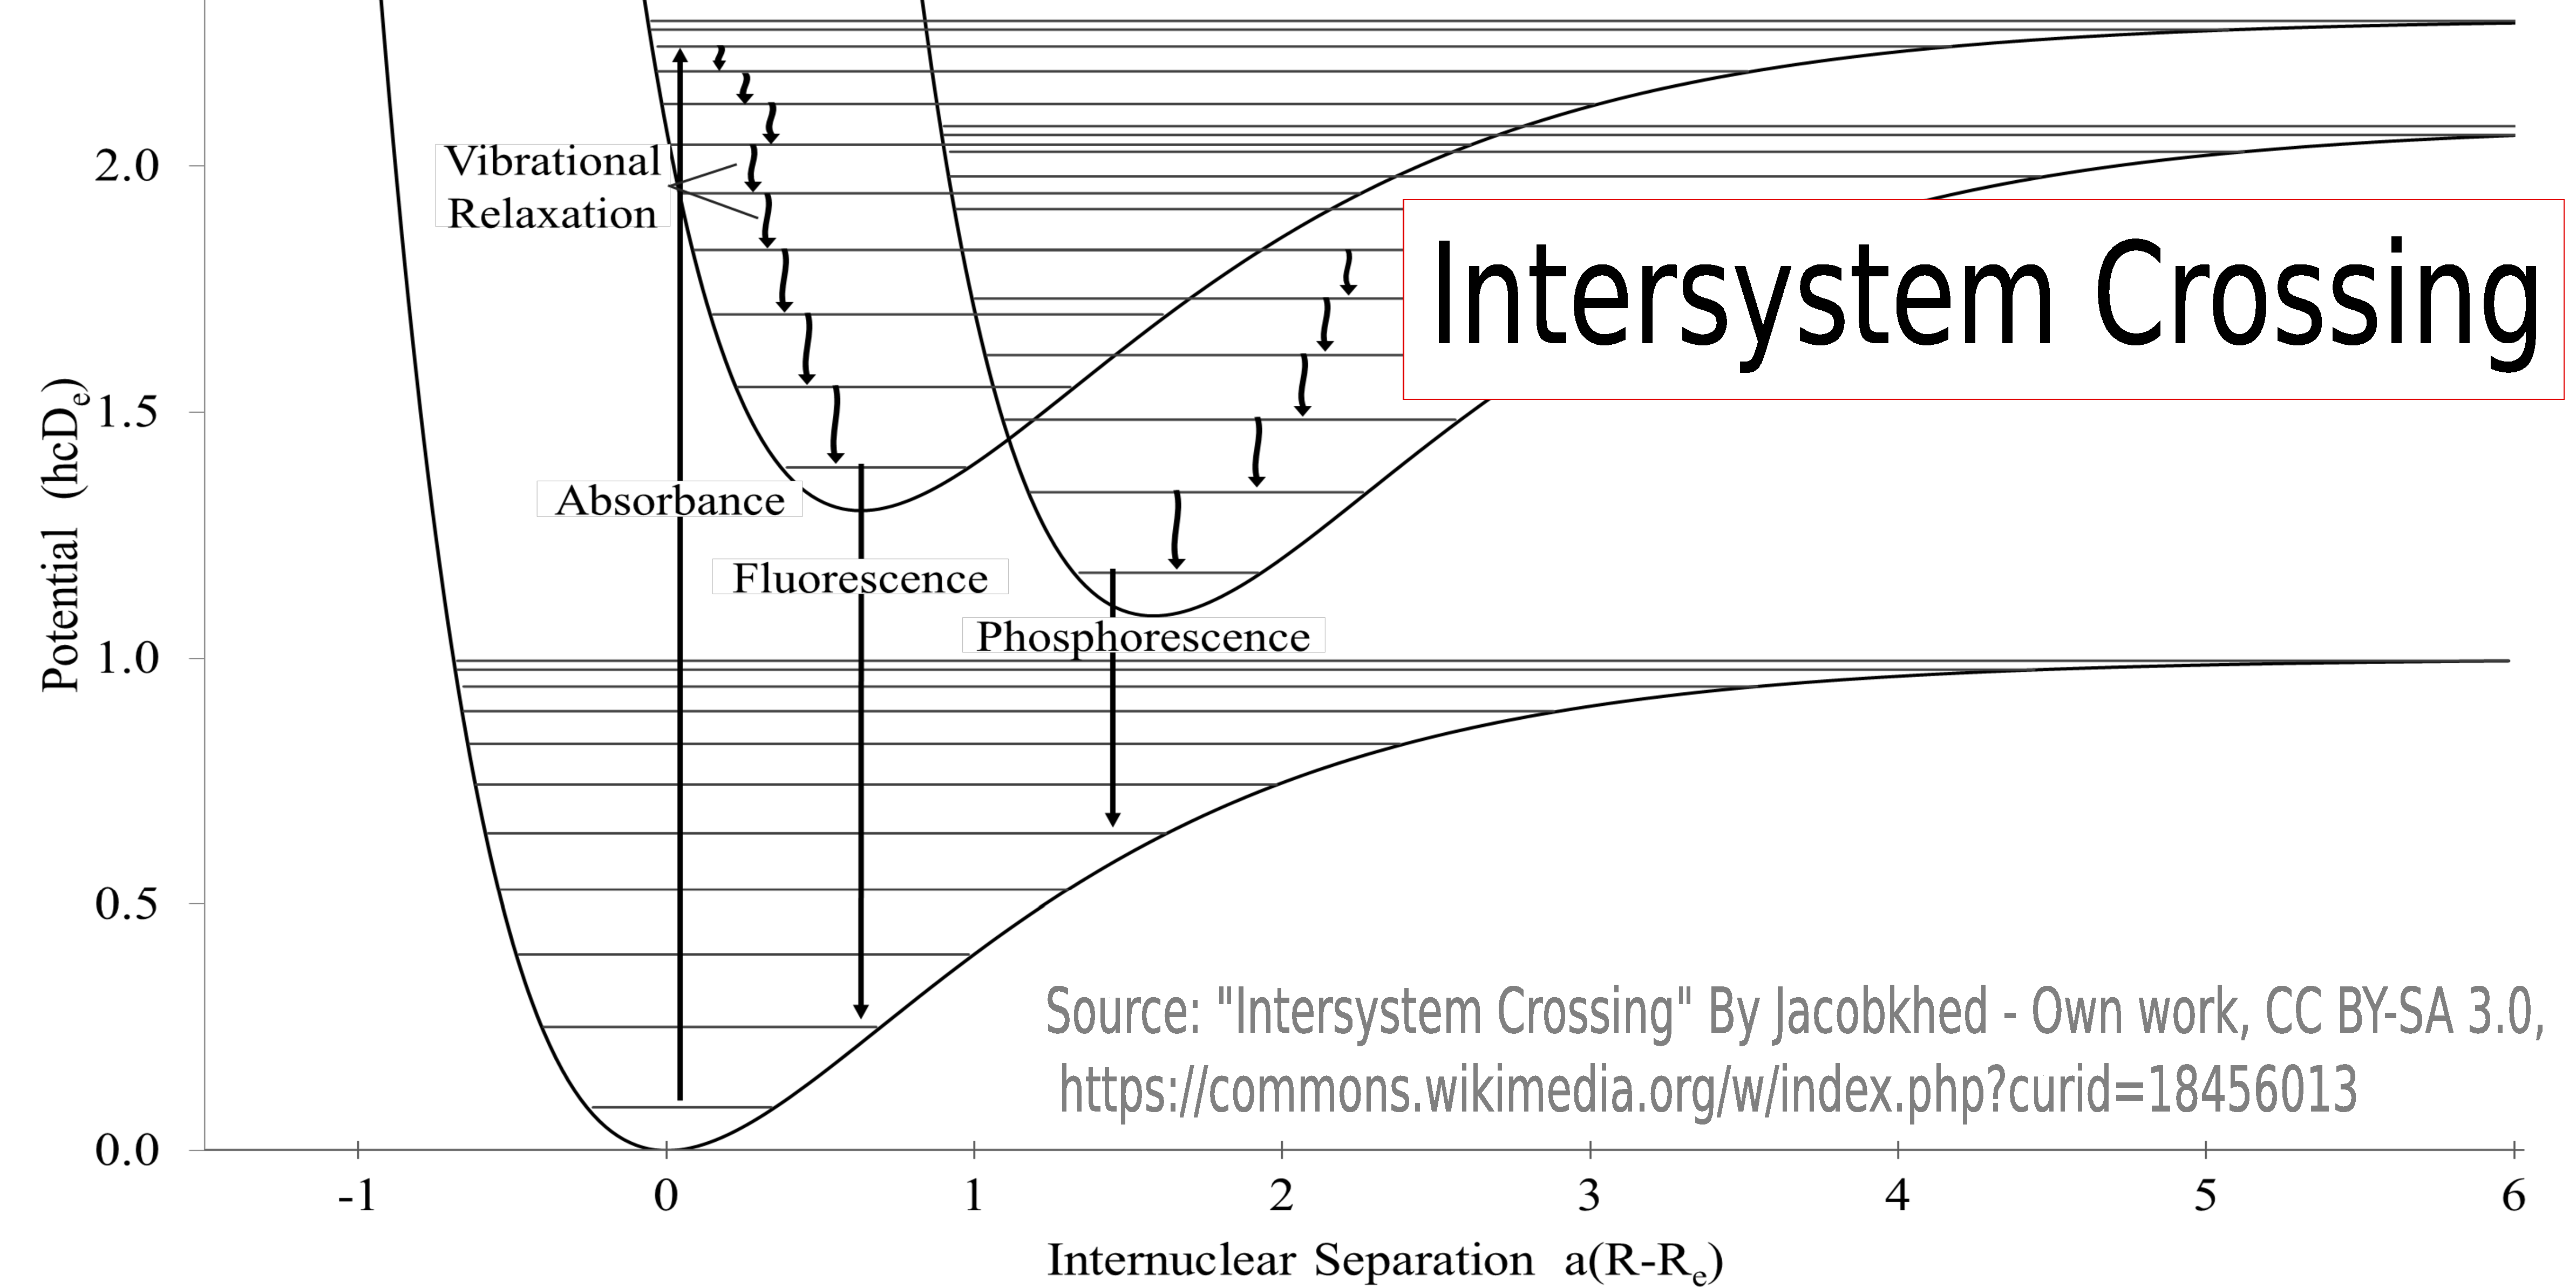
\includegraphics[width=0.9\columnwidth]{../img/SF_esq20.pdf}
	%\end{figure}
	%\begin{multicols}{2}
	%
	%\hspace{-20pt}\vspace{-20pt}
	%\begin{figure}[H]
	%\hspace{-20pt}\vspace{-20pt}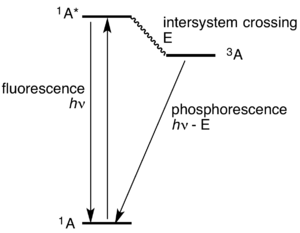
\includegraphics[width=0.7\columnwidth]{../img/SF_esq19.png}
	%\end{figure}
	%%\columnbreak
	%\footnotesize
	%\hspace{-20pt}Non-Radiatively: Singlet to Triplet state (reverse of the electron spin)\\
	%\hspace{-20pt}1- Overlap of vibrational levels\\
	%(little E loss/gain, $\sim kT$)\\
	%\hspace{-20pt}2- \textbf{Spin-Orbit Coupling}\\
	%%(Interaction with $\overrightarrow{L}$ of non-circular orbits)\\
	%%\hspace{-20pt}
	%(heavy-atom molecules and paramagnetic species)
	%
	%\end{multicols}
\end{frame}



\begin{frame}
	\frametitle{Quantification \texttt{mill}}
	
	\begin{figure}[H]
		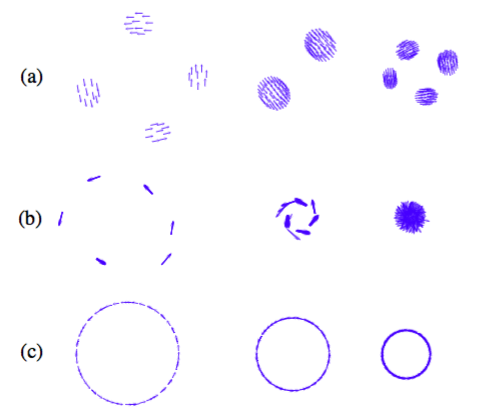
\includegraphics[width=.75\columnwidth]{./img/ClumpsRing.png}
		\caption{Catastrophic geometry. \\(a) Clumps. (b) Ring Clumping. (c) Rings.}
		\label{clumps}
	\end{figure}
	
	
	%%\begin{multicols}{2}
	%\begin{figure}[H]
	%\hspace{-10pt}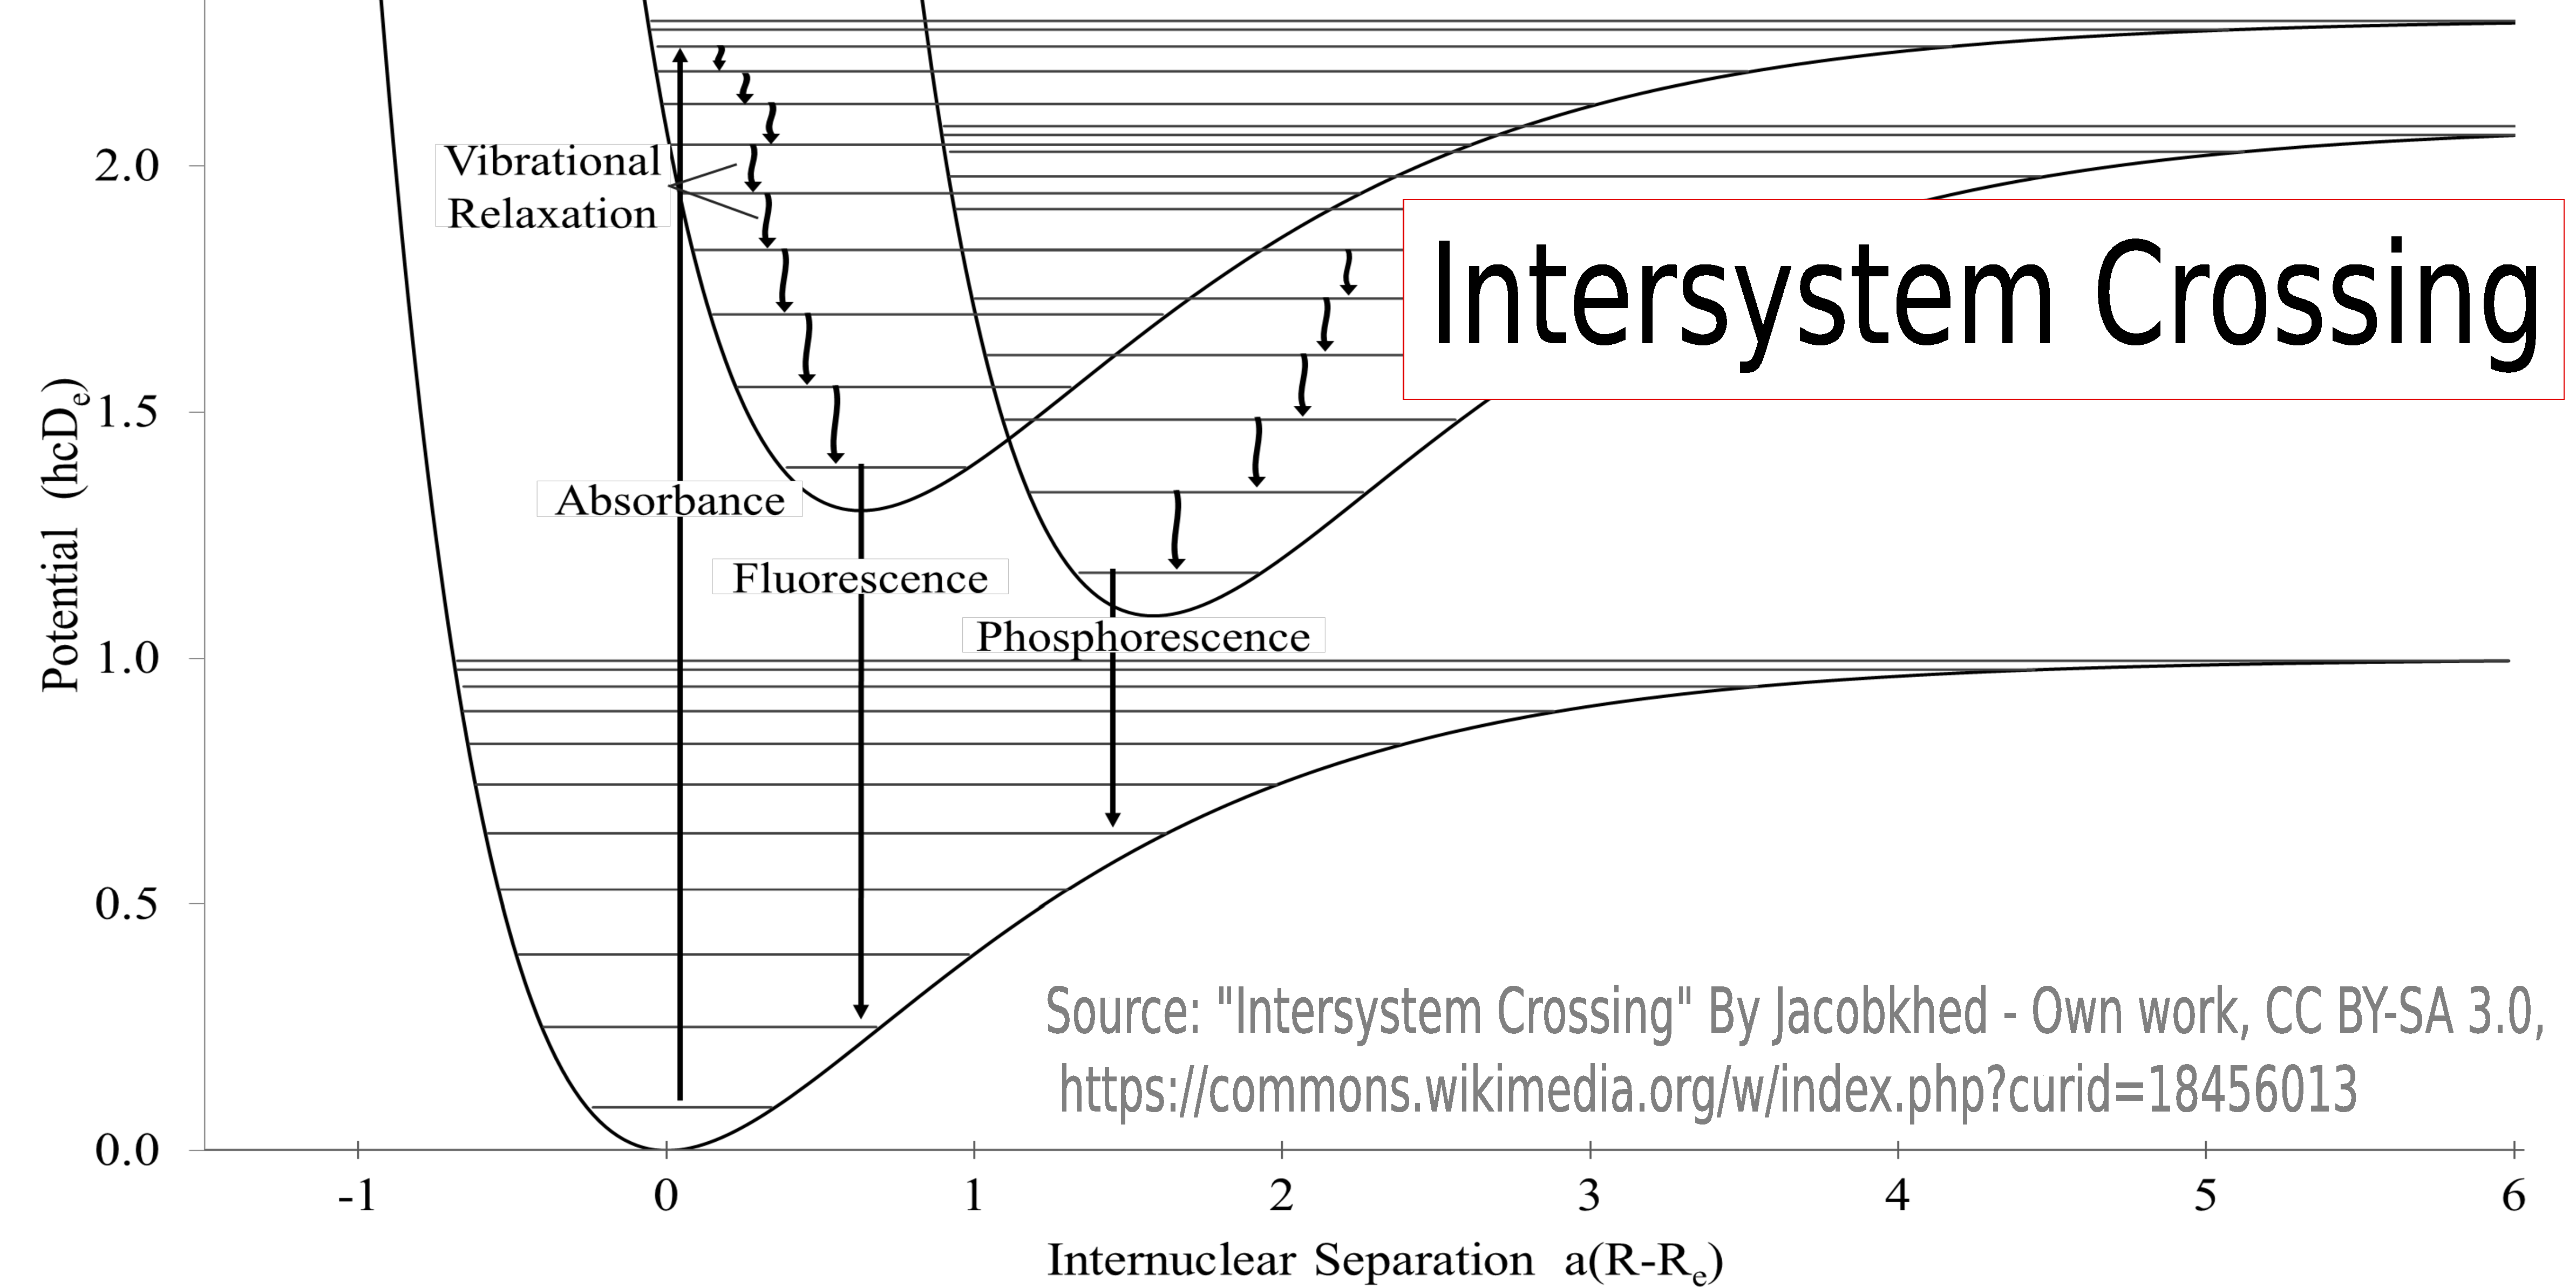
\includegraphics[width=0.9\columnwidth]{../img/SF_esq20.pdf}
	%\end{figure}
	%\begin{multicols}{2}
	%
	%\hspace{-20pt}\vspace{-20pt}
	%\begin{figure}[H]
	%\hspace{-20pt}\vspace{-20pt}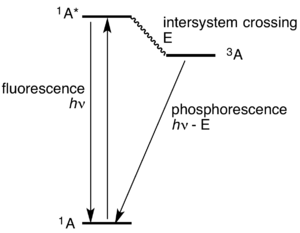
\includegraphics[width=0.7\columnwidth]{../img/SF_esq19.png}
	%\end{figure}
	%%\columnbreak
	%\footnotesize
	%\hspace{-20pt}Non-Radiatively: Singlet to Triplet state (reverse of the electron spin)\\
	%\hspace{-20pt}1- Overlap of vibrational levels\\
	%(little E loss/gain, $\sim kT$)\\
	%\hspace{-20pt}2- \textbf{Spin-Orbit Coupling}\\
	%%(Interaction with $\overrightarrow{L}$ of non-circular orbits)\\
	%%\hspace{-20pt}
	%(heavy-atom molecules and paramagnetic species)
	%
	%\end{multicols}
\end{frame}


\begin{frame}
	\frametitle{Quantification \texttt{mill}}
	
	\begin{figure}[H]
		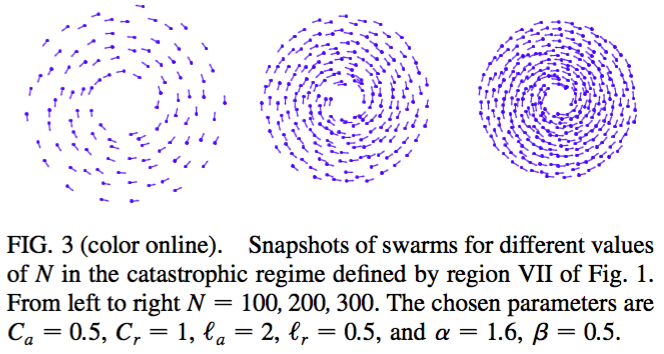
\includegraphics[width=1.\columnwidth]{./img/snapshots.png}
		%\caption{snapshots of farms for different values of \( N \) in region VII. }
		\label{snapshots}
	\end{figure}
	
	
	%%\begin{multicols}{2}
	%\begin{figure}[H]
	%\hspace{-10pt}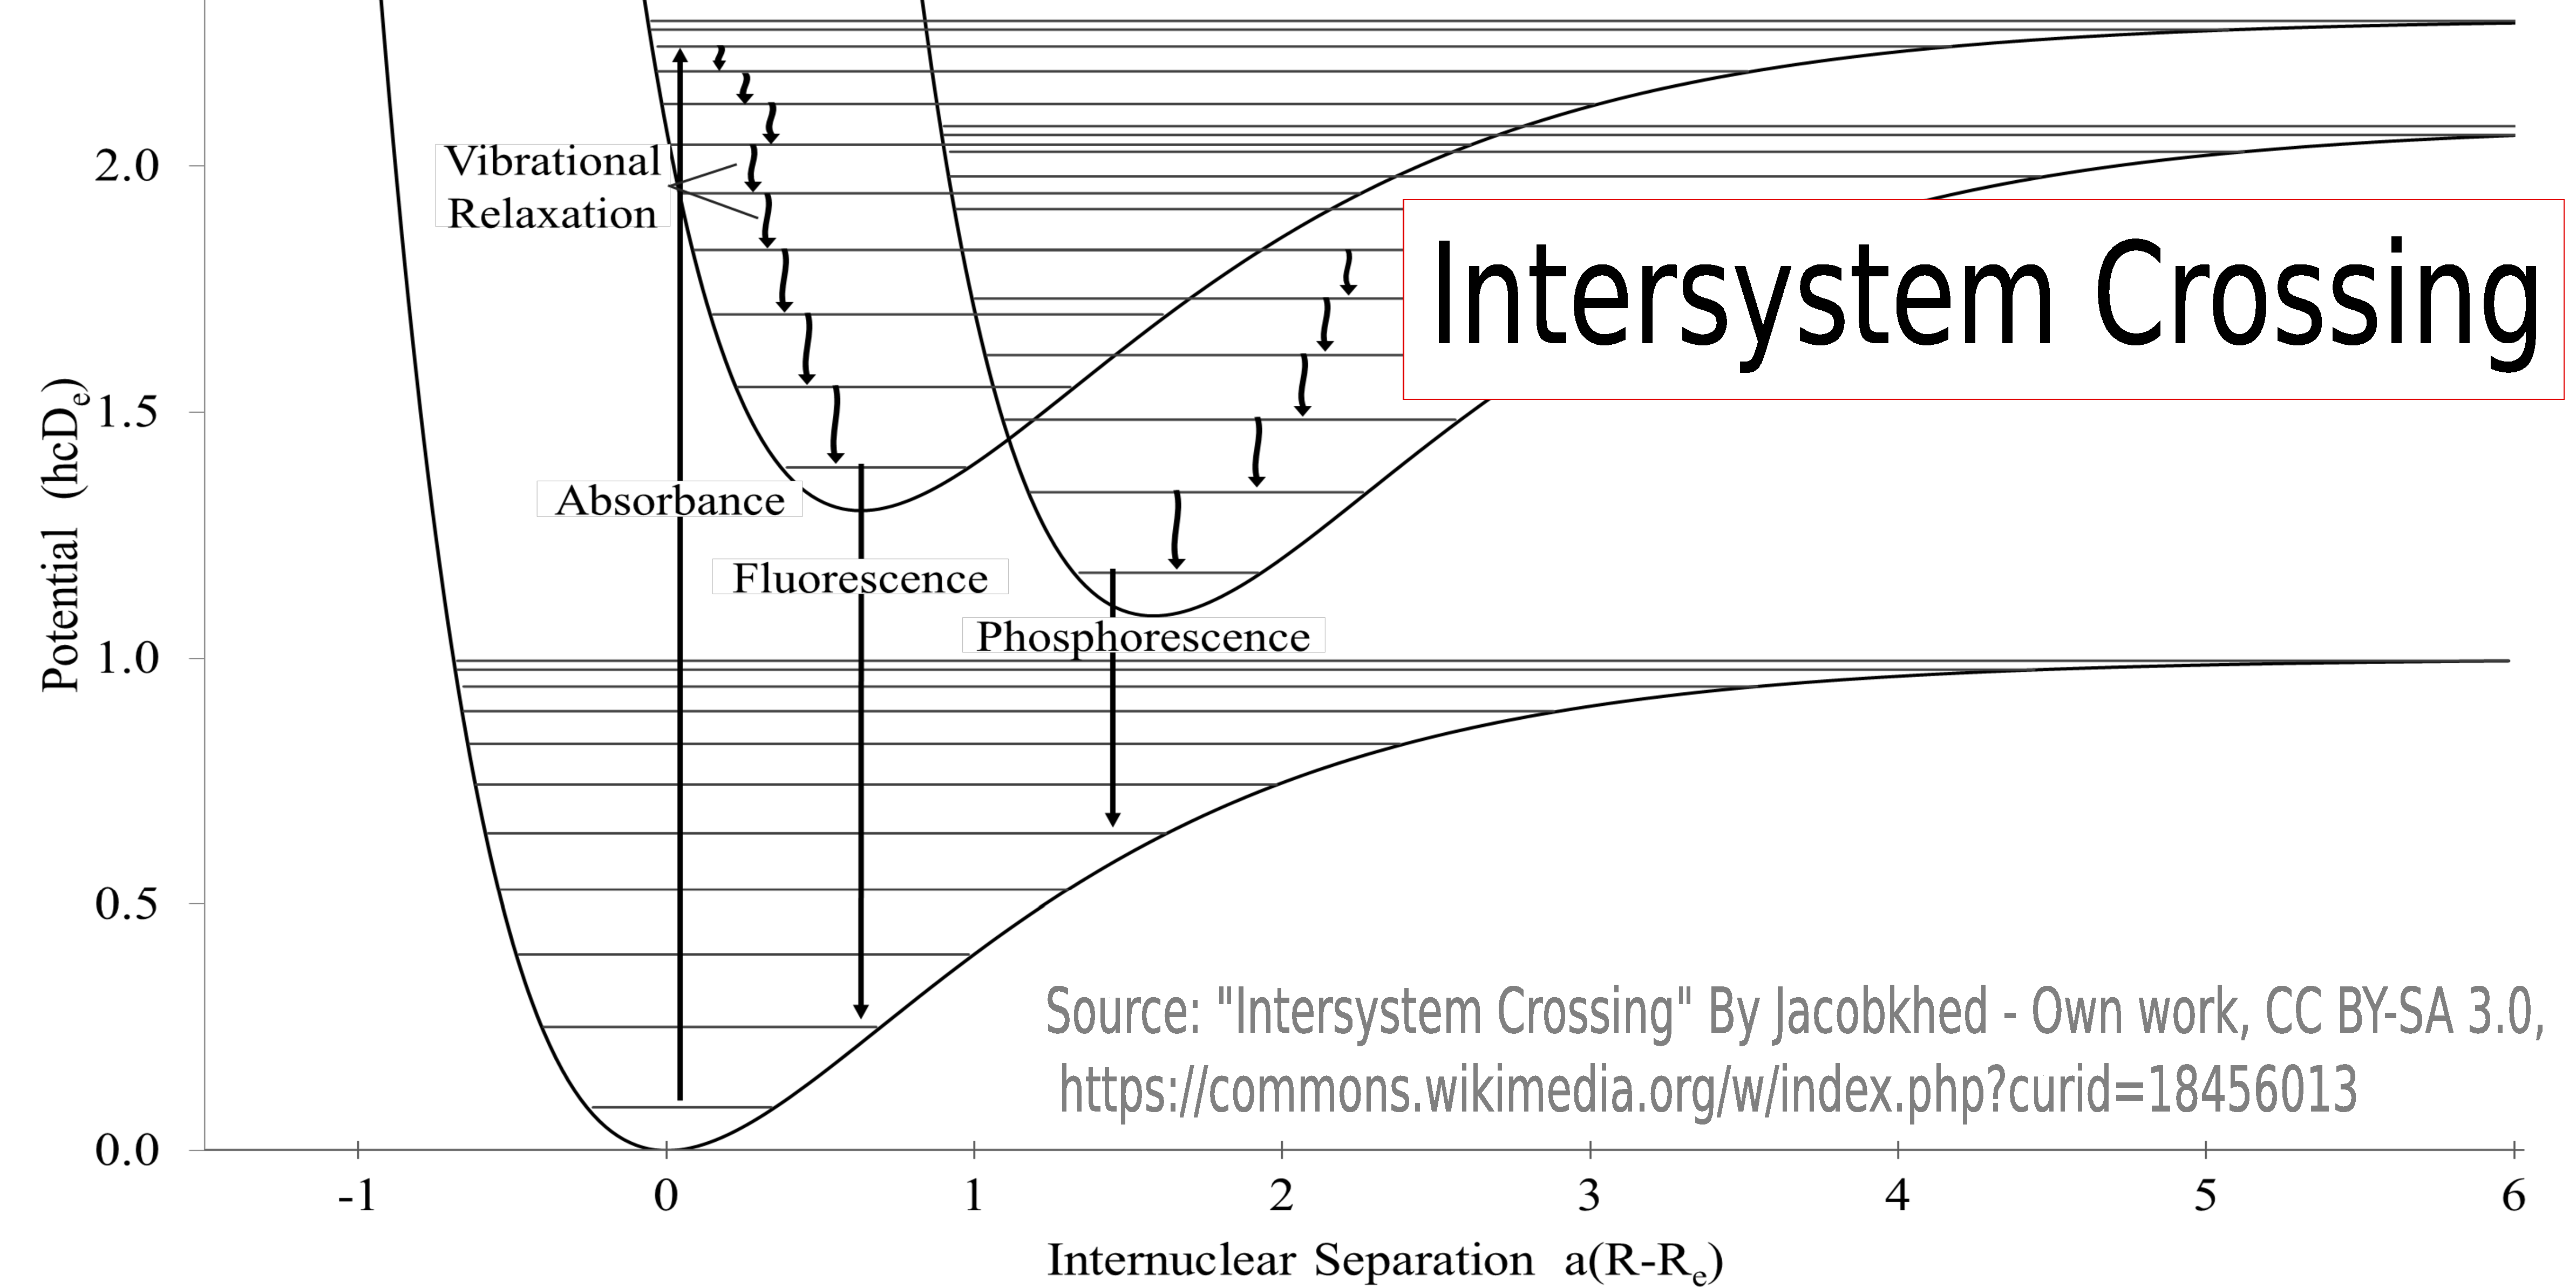
\includegraphics[width=0.9\columnwidth]{../img/SF_esq20.pdf}
	%\end{figure}
	%\begin{multicols}{2}
	%
	%\hspace{-20pt}\vspace{-20pt}
	%\begin{figure}[H]
	%\hspace{-20pt}\vspace{-20pt}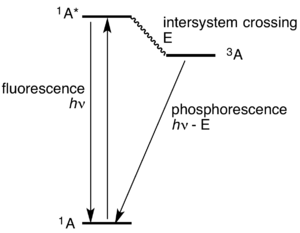
\includegraphics[width=0.7\columnwidth]{../img/SF_esq19.png}
	%\end{figure}
	%%\columnbreak
	%\footnotesize
	%\hspace{-20pt}Non-Radiatively: Singlet to Triplet state (reverse of the electron spin)\\
	%\hspace{-20pt}1- Overlap of vibrational levels\\
	%(little E loss/gain, $\sim kT$)\\
	%\hspace{-20pt}2- \textbf{Spin-Orbit Coupling}\\
	%%(Interaction with $\overrightarrow{L}$ of non-circular orbits)\\
	%%\hspace{-20pt}
	%(heavy-atom molecules and paramagnetic species)
	%
	%\end{multicols}
\end{frame}


\begin{frame}
	\frametitle{Quantification \texttt{mill}}
	
	\begin{figure}[H]
		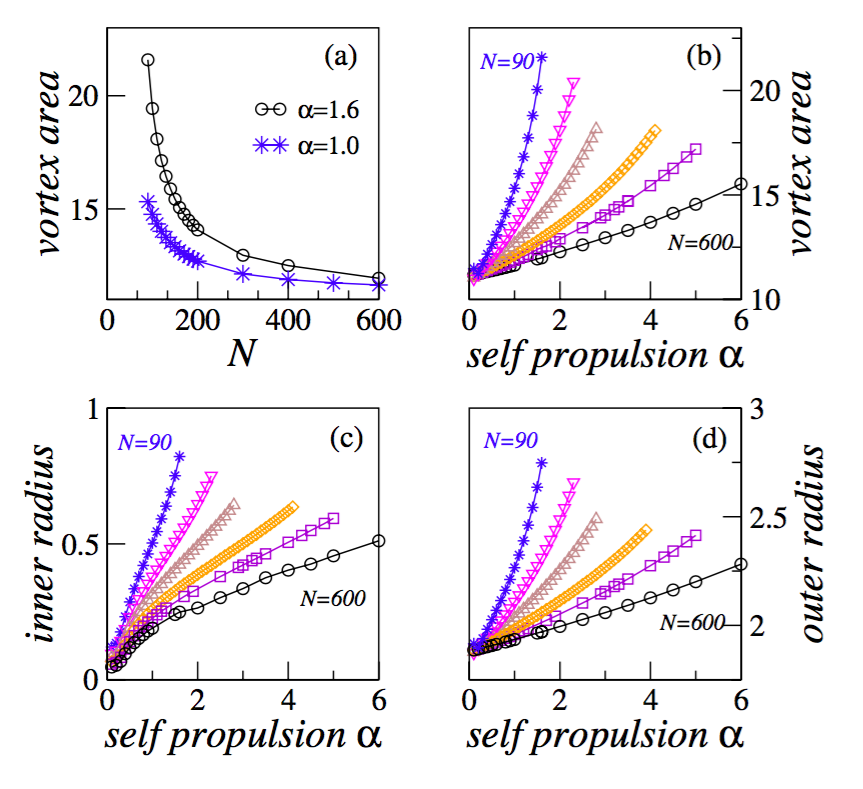
\includegraphics[width=.7 \columnwidth]{./img/vortexScaling.png}
		\caption{Vortex scaling for the catastrophic Morse potential.}
		\label{vortexScaling}
	\end{figure}
	
	
	%%\begin{multicols}{2}
	%\begin{figure}[H]
	%\hspace{-10pt}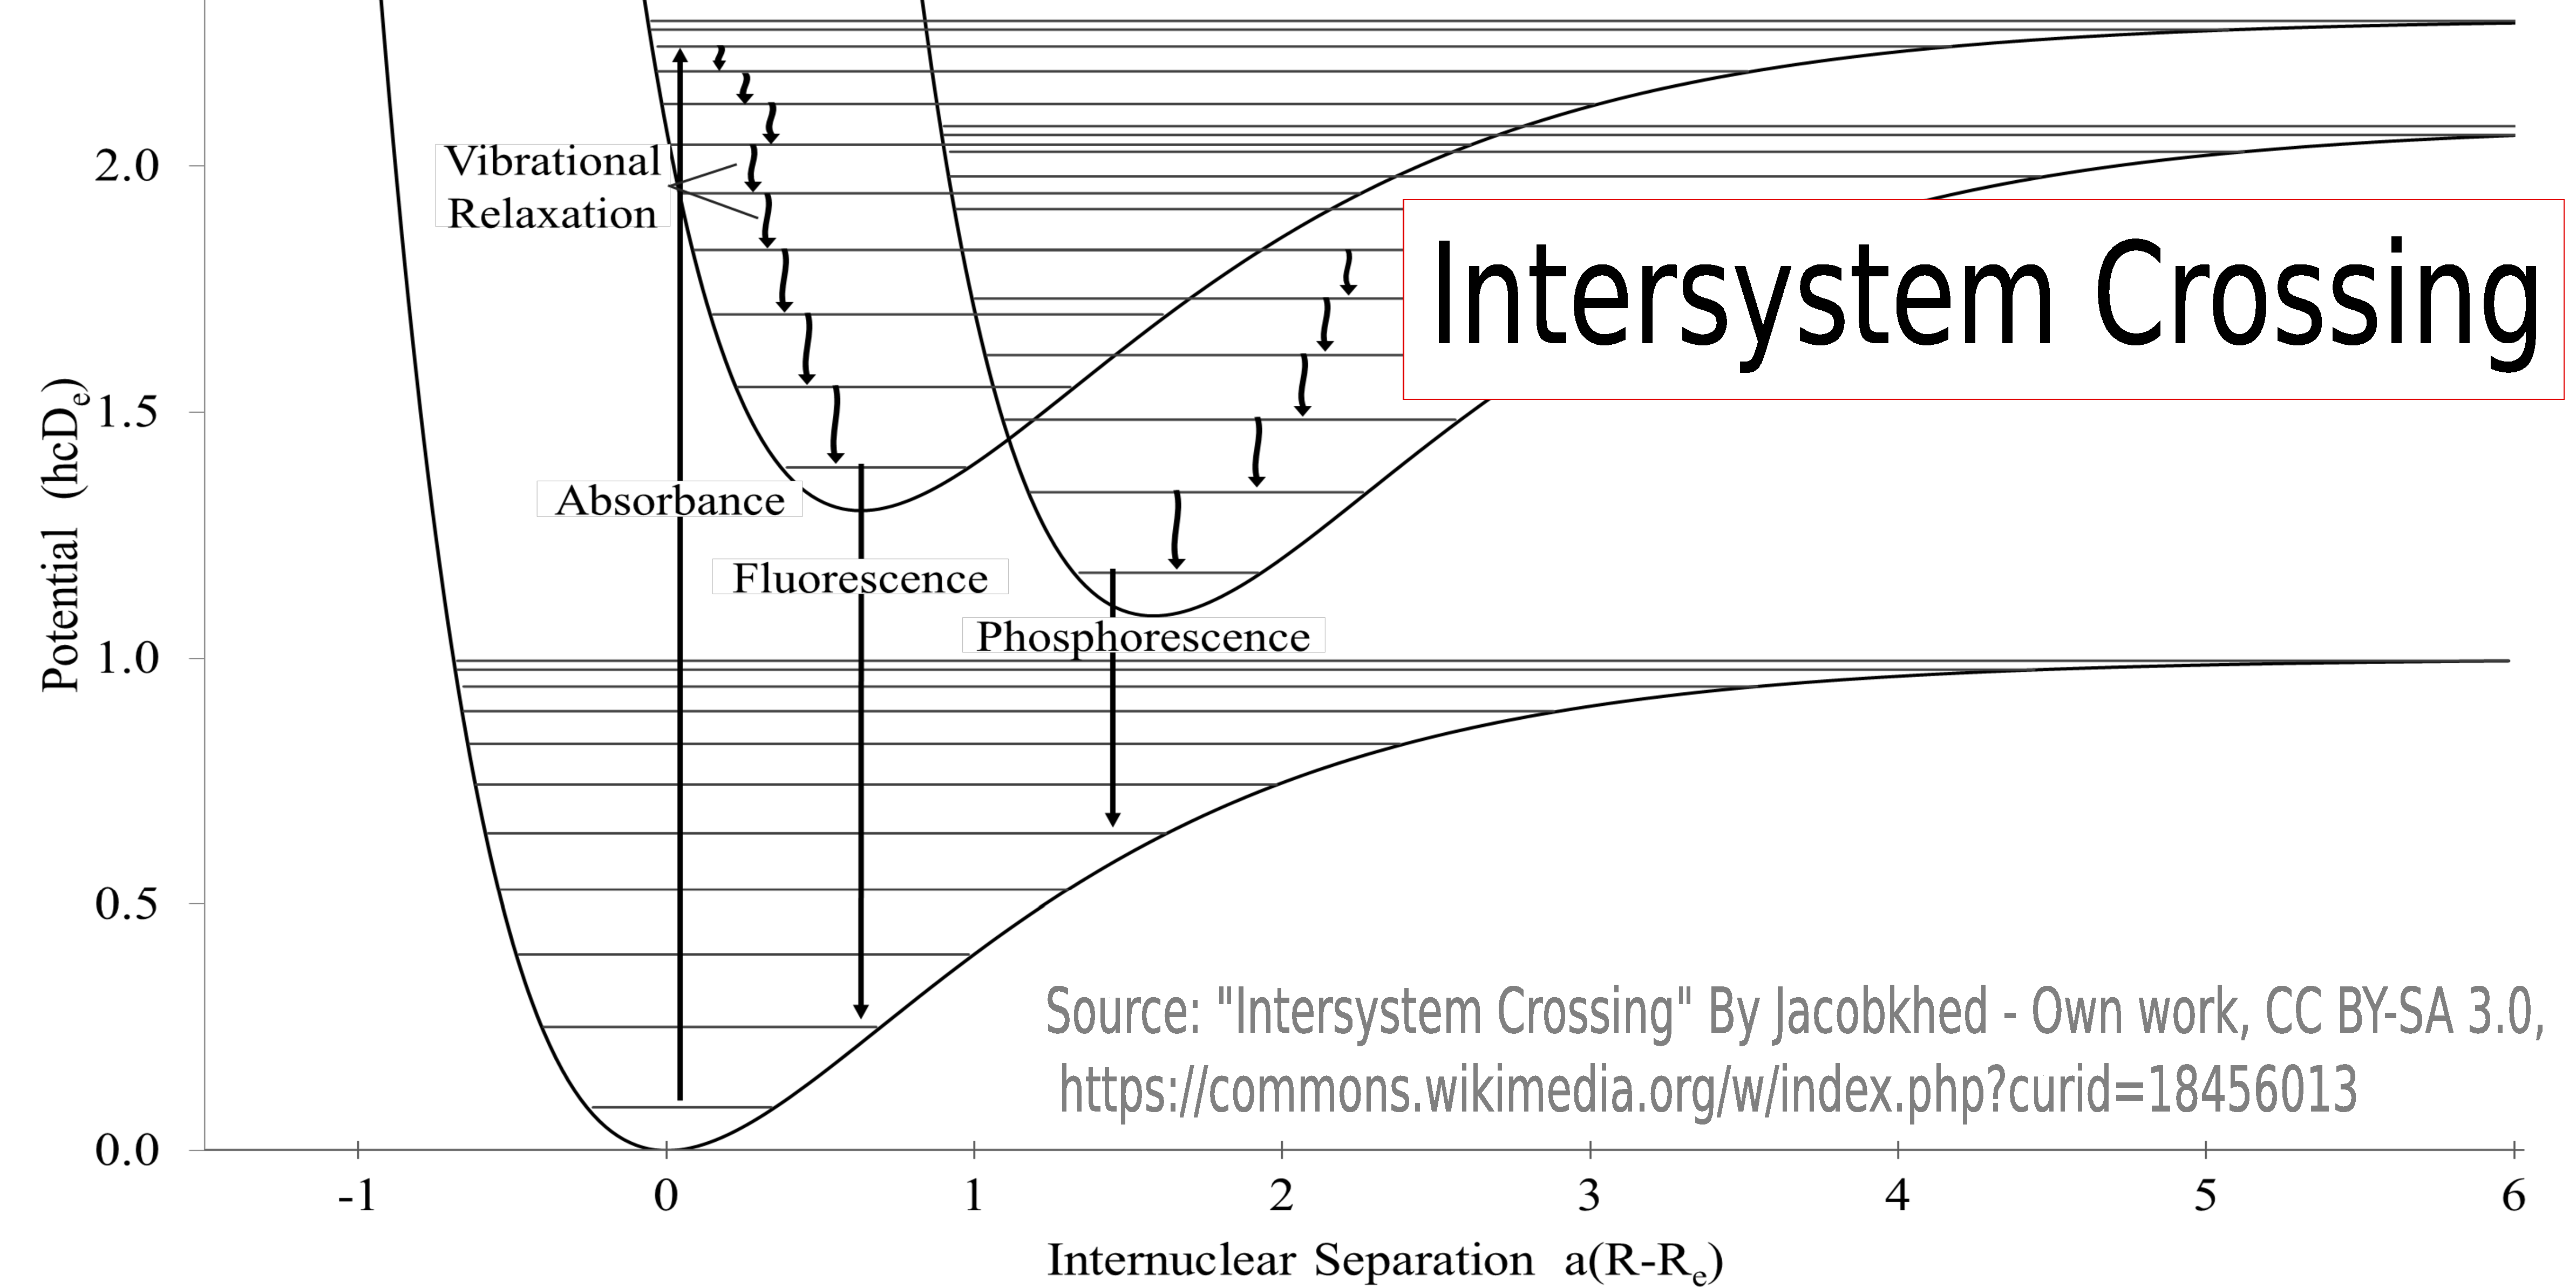
\includegraphics[width=0.9\columnwidth]{../img/SF_esq20.pdf}
	%\end{figure}
	%\begin{multicols}{2}
	%
	%\hspace{-20pt}\vspace{-20pt}
	%\begin{figure}[H]
	%\hspace{-20pt}\vspace{-20pt}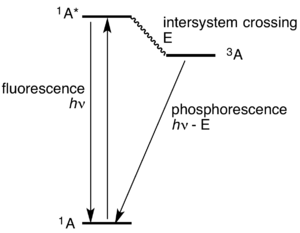
\includegraphics[width=0.7\columnwidth]{../img/SF_esq19.png}
	%\end{figure}
	%%\columnbreak
	%\footnotesize
	%\hspace{-20pt}Non-Radiatively: Singlet to Triplet state (reverse of the electron spin)\\
	%\hspace{-20pt}1- Overlap of vibrational levels\\
	%(little E loss/gain, $\sim kT$)\\
	%\hspace{-20pt}2- \textbf{Spin-Orbit Coupling}\\
	%%(Interaction with $\overrightarrow{L}$ of non-circular orbits)\\
	%%\hspace{-20pt}
	%(heavy-atom molecules and paramagnetic species)
	%
	%\end{multicols}
\end{frame}

%\begin{frame}
%  \frametitle{Singlet Fission: Process I}
%%\begin{multicols}{2}
%%\vspace{-10pt}
%%\begin{figure}[H]
%%%centering
%%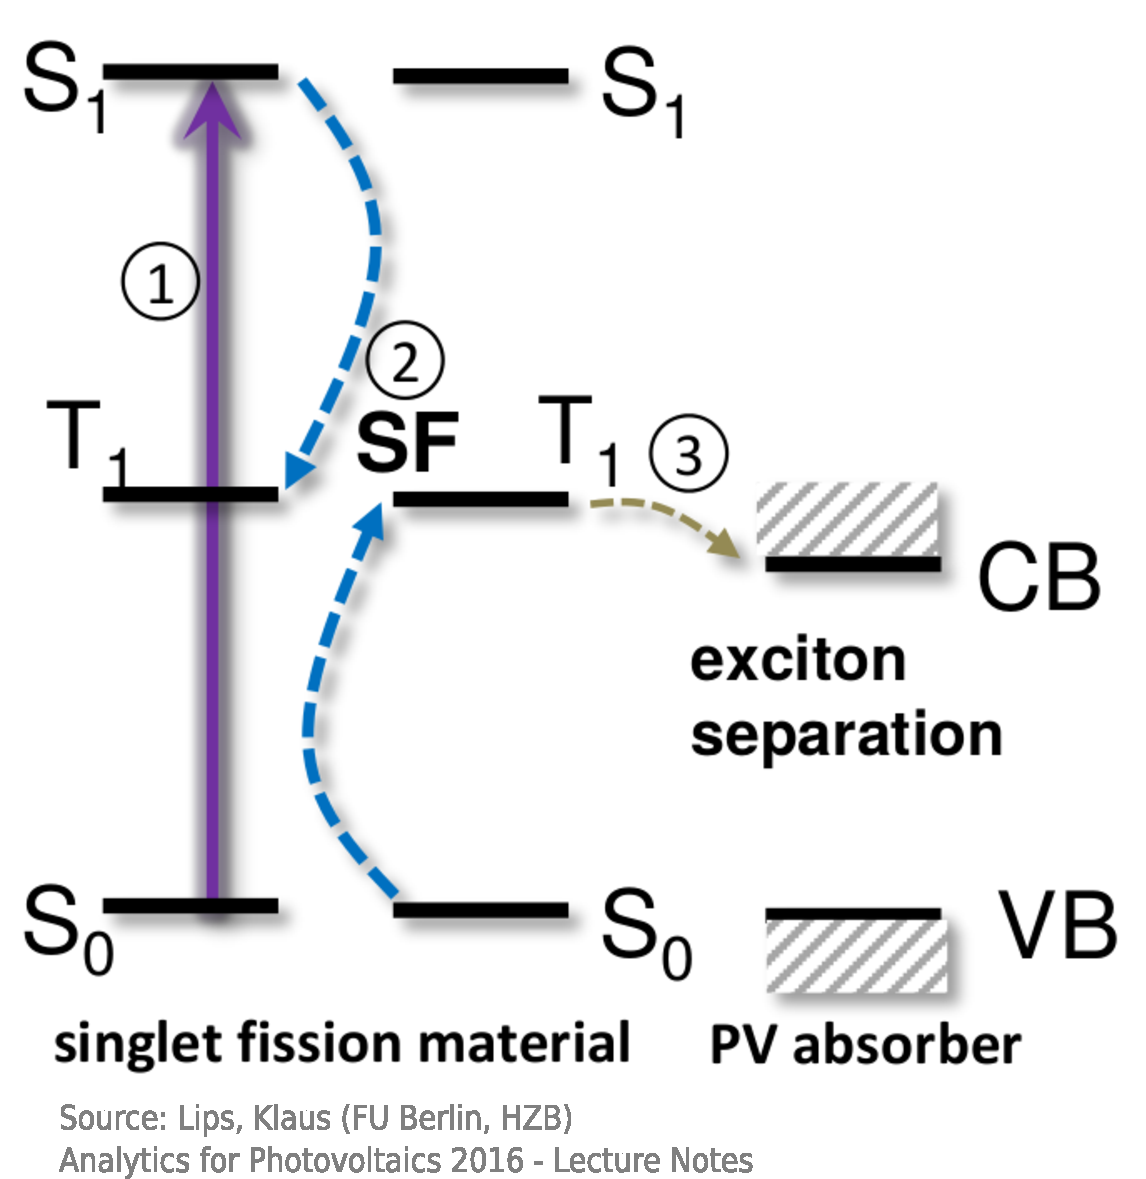
\includegraphics[width=1.1\columnwidth]{../img/SF_esq11.pdf}
%%\end{figure}
%%\small
%%\hspace{-15pt}- $S_1$ controls optical properties\\
%%\hspace{-15pt}- $T_1$ controls electrical properties\\
%%
%%\begin{figure}[H]
%%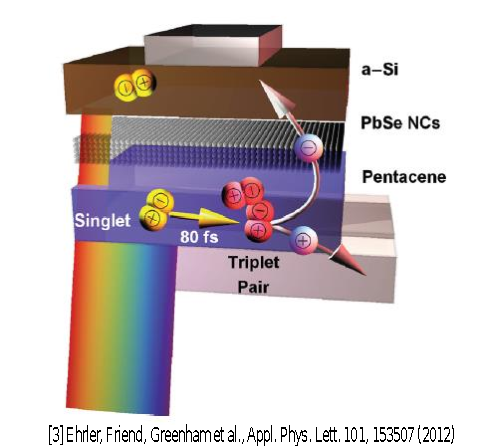
\includegraphics[width=1.2\columnwidth]{../img/SF_esq3.pdf}
%%\end{figure}
%%\small
%%\hspace{-15pt}- Fission Probability\\
%%\hspace{-15pt}- Triplet-state lifetime\\
%%\hspace{-15pt}- Successful (2x) charge separation
%%\end{multicols}
%
%
%\end{frame}
%
%\begin{frame}
%\frametitle{Singlet Fission: Process II}
%%
%%\begin{figure}[H]
%%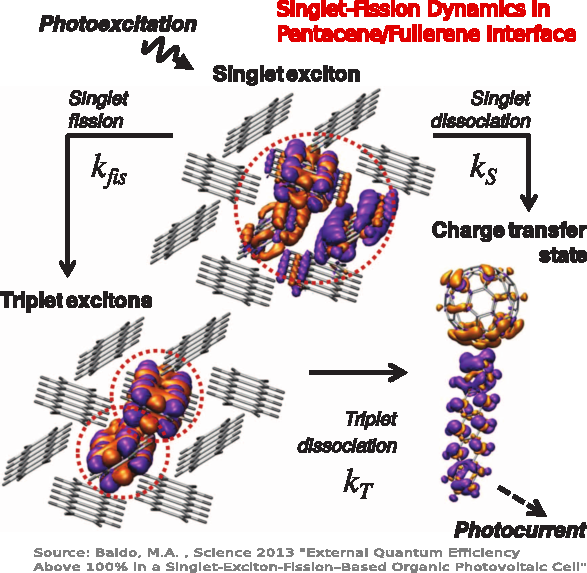
\includegraphics[width=0.7\columnwidth]{../img/SF_esq18.pdf}
%%\end{figure}
%%%Calculationsofsingletandtripletexcitonsandcharge
%%%transferstatesatthepentacene/fullereneinterfaceareshown,withthepurple(orange)densityindicating
%%%whereless(more)electrondensityisfoundintheexcitedstate.Thedelocalizedsingletexcitonandtwo
%%%localizedtripletexcitonsarecircledinred.Thelosspathwayforsingletexcitonsisdirectdissociationinto
%%%chargebeforesingletexcitonfission.
%
%\end{frame}
%
%
%\begin{frame}
%  \frametitle{Singlet Fission: Material Example}
%%\vspace{-10pt}
%%\hspace{-30pt}
%%\begin{figure}[H]
%%%centering
%%\hspace{-10pt}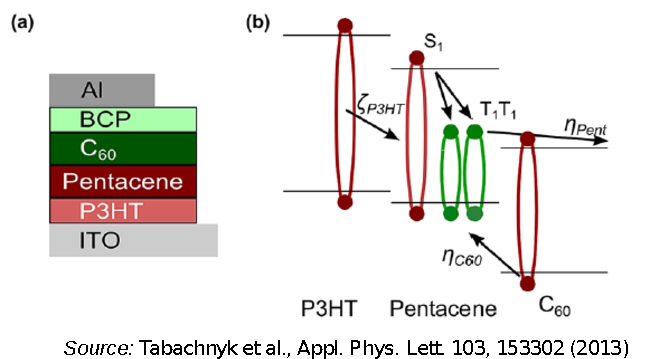
\includegraphics[width=.7\columnwidth]{../img/SF_esq4.pdf}
%%\end{figure}
%%
%%%\columnbreak
%%\begin{multicols}{2}
%%
%%\begin{figure}[H]
%%%centering
%%\vspace{-40pt}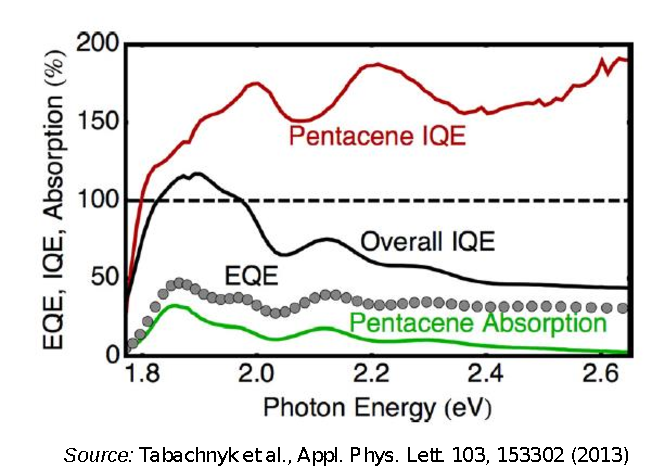
\includegraphics[width=1\columnwidth]{../img/SF_esq5.pdf}
%%\end{figure}
%%
%%%\hspace{40pt}(different side-groups)\\
%%%\hspace{40pt}(Hanna, Nozik) tetracene, anthracene, other polyacene crystals
%%\begin{figure}[H]
%%%centering
%%\vspace{-40pt}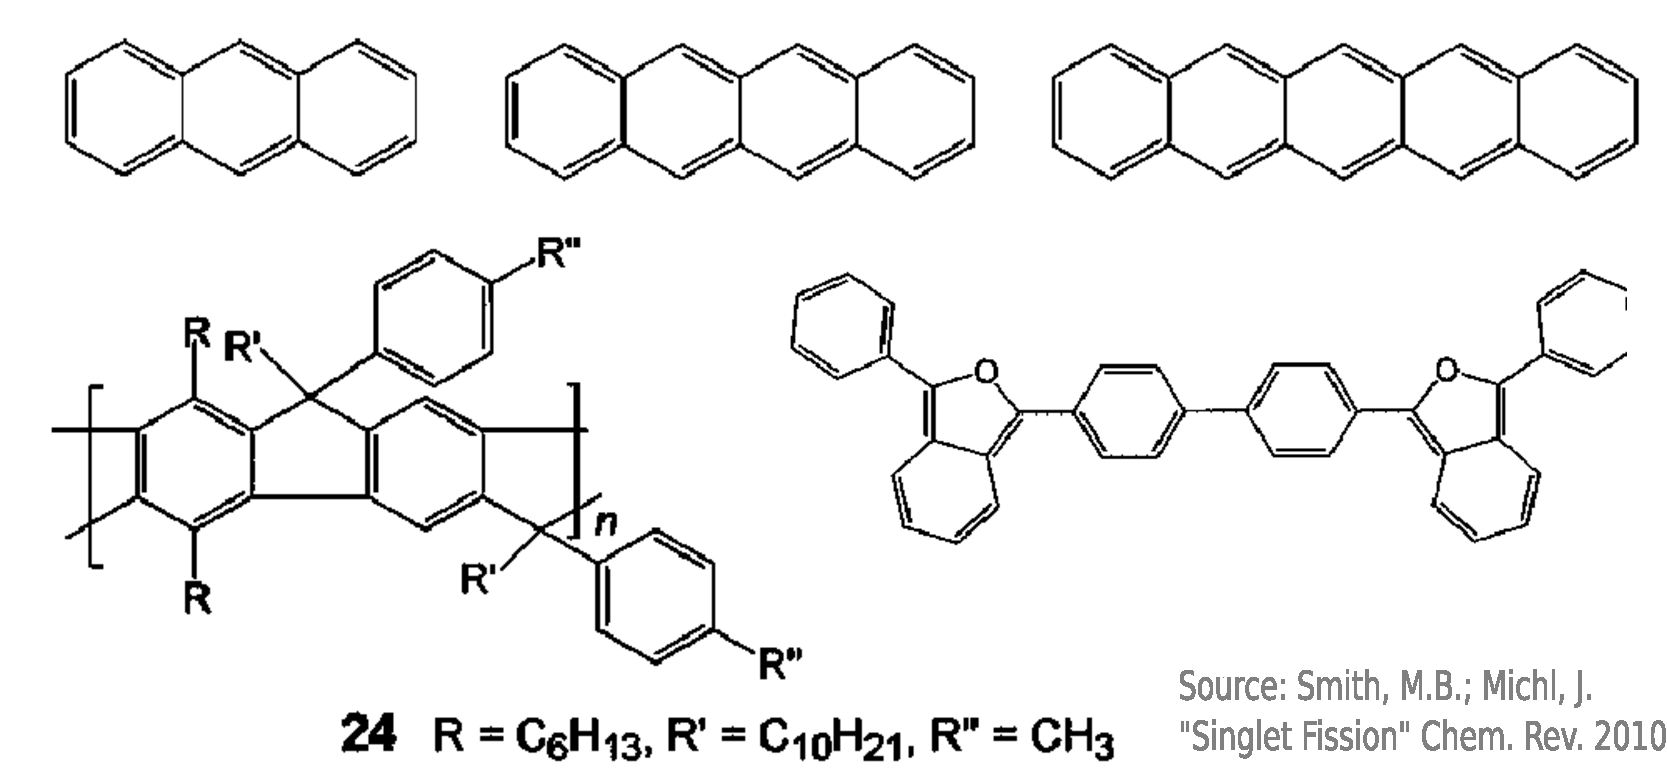
\includegraphics[width=1\columnwidth]{../img/SF_esq21.pdf}
%%\end{figure}
%%\vspace{-15pt}\footnotesize Tetracene, Pentacene, Anthracene\\
%%
%%
%%\end{multicols}
%
%\end{frame}
%
%
%\begin{frame}
%  \frametitle{Singlet Fission: Detection Techniques}
%%\normalsize
%%%\begin{multicols}{2}
%%\begin{itemize}
%%\item Photo-Luminescence (t-resolved)
%%\item Magneto-Optical Techniques\\
%%\hspace{10pt}\footnotesize (change in Photo-Luminescence with $\overrightarrow{B}$ field through Zeeman interaction)
%%\normalsize
%%\item Electron-Paramagnetic Resonance (EPR) and transient EPR\\
%%\hspace{10pt}\footnotesize (at FUB/HZB with TIPS-tetracene - soluable and change in E-states)
%%\end{itemize}
%%\begin{figure}[H]
%%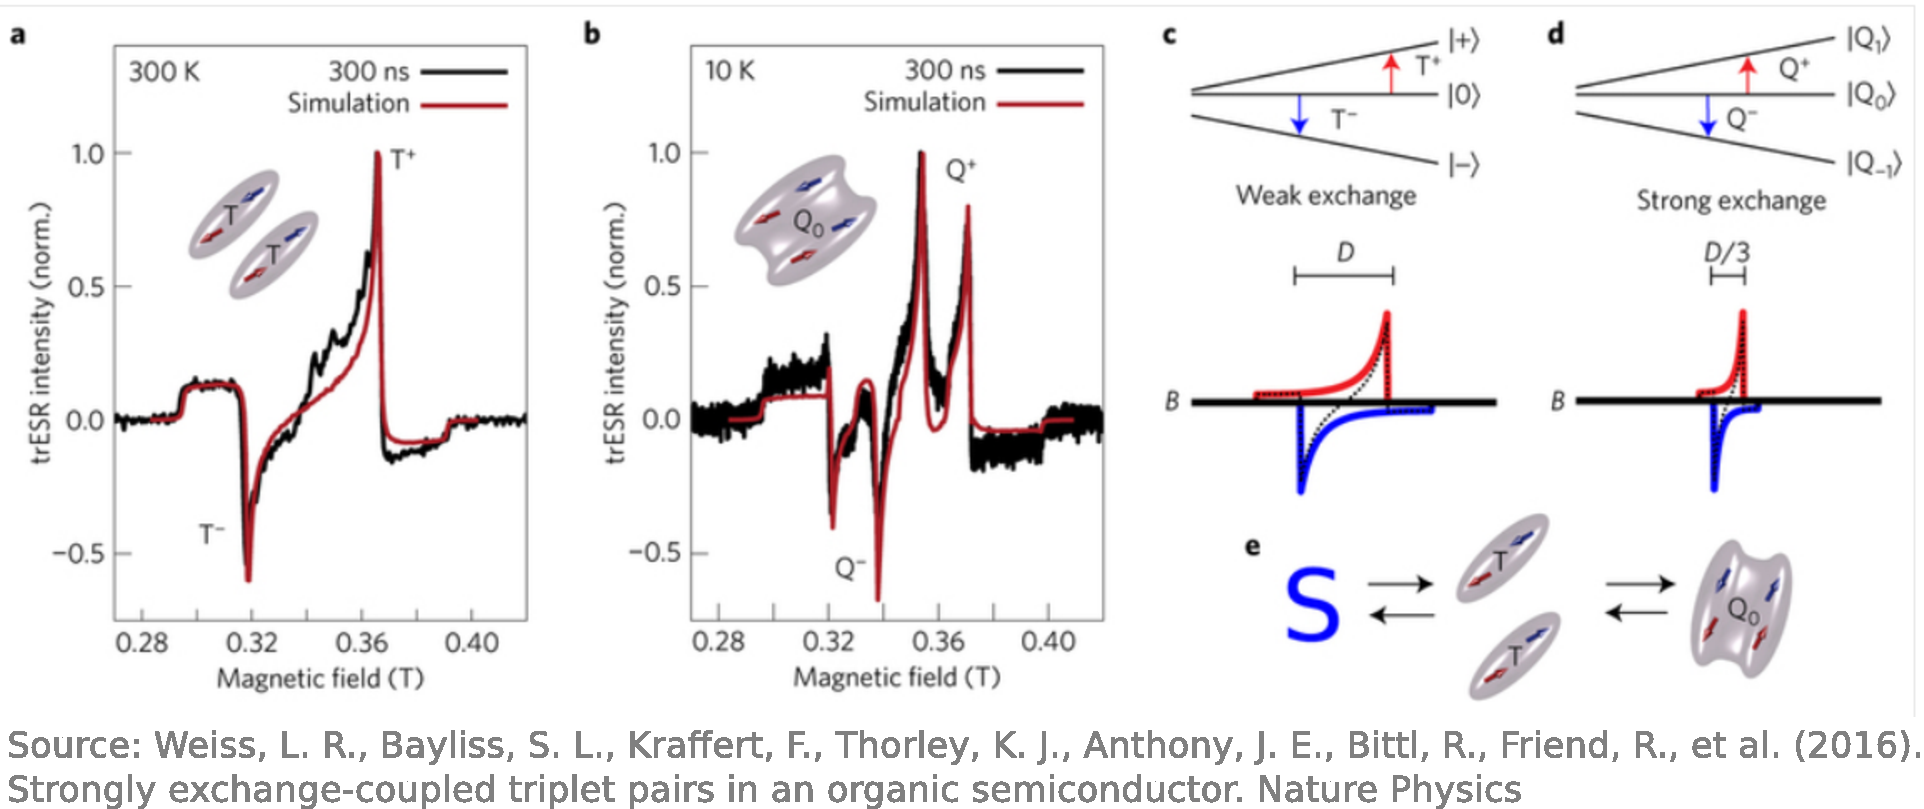
\includegraphics[width=1\columnwidth]{../img/SF_HZB.pdf}
%%\end{figure}
%%
%%%\end{multicols}
%
%\end{frame}
%
%
%\begin{frame}
%  \frametitle{Singlet Fission: Trends \& Challenges}
%%%\begin{multicols}{2}
%%\vspace{-10pt}
%%\underline{Application}\\
%%- tandem PV - SF(b)/M2(t): $47,7\%$ (Highest efficiency!)\\
%%
%%%\end{multicols}
%%\underline{Challenges:}
%%
%%\begin{itemize}
%%\item Cost \& Long-term stability in sunlight
%%\item Matching E-levels for fast (but low potential-loss) charge separation/transfer;
%%\item Preventing premature charge injection from first $S_1$ while assuring efficient charge injection from $T_1$
%%\item Max SF rate, min TTA rate; max absorption at all $E>E_g$
%%\item Neighbouring molecules coupled in pair or higher agregates; \textbf{strong} coupling for fast SF
%%\item Independent behaviour of both $T_1$; \textbf{weak} coupling for efficient charge separation
%%\end{itemize}
%
%\end{frame}
%
%
%
%\begin{frame}
%  \frametitle{Aknowledgements}
%%\begin{itemize}
%%\item Thanks to Klaus Lips and Rowan McQueen for the complete and well organized course "Analytics for Photovoltaics" (WS 2016) wherefrom I could have a lot of backup information and material
%%\item Thanks to the EPR department of HZB - Alexander Schnegg, Shane Bonke - where I was allowed to do an Internship on the technique's field and contact more with the Solar Cells and Solar Fuels topics
%%%\item Local defect detection
%%\end{itemize}
%%\begin{figure}[H]
%%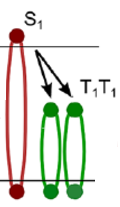
\includegraphics[width=0.15\columnwidth]{../img/SF_linda.pdf}
%%\end{figure}
%
%\end{frame}


\end{document}


